
\documentclass[xcolor={dvipsnames}]{beamer}
\usepackage{amsmath}
% \usepackage{beamerthemesplit} // Activate for custom appearance
\usepackage{hyperref}
\usepackage{ragged2e}
\usepackage{amssymb}
\usepackage{verbatim}
\usepackage{lmodern}
\usepackage{color}



\title{Non-Negative Matrix Factorization}
\author{Schwartz}
\date{\today}



\begin{document}



\frame{\titlepage}


\frame
{
\frametitle{How do you make a data scientist?}

\begin{figure}
\hspace*{.3in}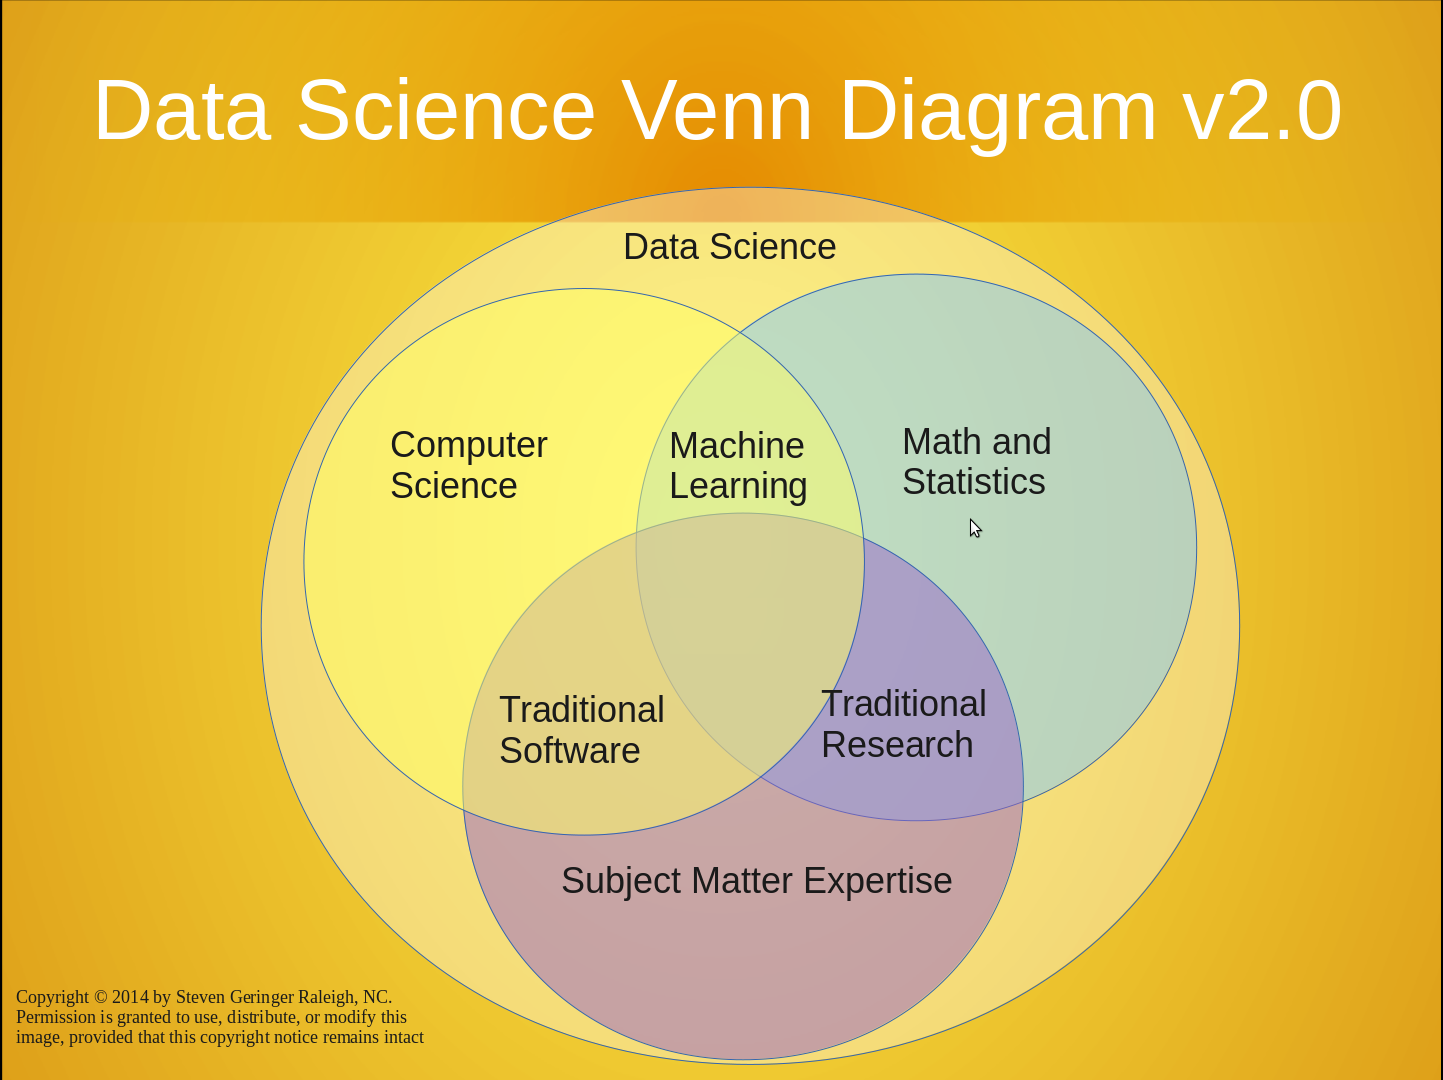
\includegraphics[width=3in]{stuff/ds_venn.png} \\${}$\\
\end{figure}
\vspace{-4em}

\tiny
\noindent \begin{columns}
\hspace*{-.7in}
\begin{column}{1\textwidth}
\begin{table}
\begin{tabular}{l|cccccccc}
& Numerical &  Scripting & Inference & Predictive  &  Business & Creative & Problem& ? \\
 &Literacy &   Coding & Estimation &  Modeling &  Acumen &  Thinking & Solving& ? \\\hline
Mathematics Degree & \\ 
Statistics Degree & \\
Economics Degree & \\
Computer Science Degree & \\
Data Science Immersive & \\
Independent Self Study &  \\
Workshops and Lectures &  \\
Community Engagement & \\
? \\
\end{tabular}
\end{table}
\end{column}
\end{columns}

}

\frame
{
\frametitle{Objectives}

\LARGE 
\begin{itemize}
\item NMF 
\begin{itemize}
\Large
\item versus SVD
\item non-negative 
\item parts-based model 
\end{itemize}
\item Uses 
\begin{itemize}
\Large
\item learn/interpret latent reduced dimensionality features driving data 
\item soft cluster samples by latent features
\end{itemize}
\item Estimating NMF
\begin{itemize}
\Large
\item gradient descent
\item alternating least squares (ALS)
\item multiplicative updating
\end{itemize}

\end{itemize}

}


\frame
{
\frametitle{What is NMF?}


\emph{Singular Value Decomposition (SVD)}: 
\LARGE
\begin{align*} % requires amsmath; align* for no eq. number
\underset{n\times p}{X}  = {}& \underset{n\times n}{U}\;\;\underset{n\times p}{\Sigma} \;\; \underset{p\times p}{V}^T \\
\approx {}&\underset{n\times \textcolor{red}{k}}{U}\;\;\underset{\textcolor{red}{k \times k}}{\Sigma} \;\; \underset{\textcolor{red}{k}\times p}{V}^T 
\end{align*}

\onslide<2->{
\normalsize
\emph{Non-Negative Matrix Factorization (NMF)}: 
\LARGE
\begin{align*} 
\underset{n\times p}{X} \approx{}& \underset{n \times \textcolor{red}{k}}{W}\;\;\underset{\textcolor{red}{k} \times p}{H}\\
{}&  \textcolor{gray}{ \textcolor{gray}{X_{ij}, W_{i'j'}, H_{i^*j^*} }   \geq 0}
\end{align*}
}

\normalsize
\vspace{-.75em}
\onslide<3->{\textcolor{NavyBlue}{So NMF is just SVD\\ -- just drop the middle matrix and keep all the numbers positive}}
\vspace{.25em}
}



\frame
{
\frametitle{$\geq 0$ }

Keep all the numbers positive why? \onslide<3->{\textcolor{Maroon}{Because we can}}

\vspace{-2em}

\begin{columns}
\begin{column}{.6\textwidth}


\normalsize 

\begin{table}
\begin{tabular}{c|c|c|c|c|}
Scores & item 1 & item 2 & $\cdots\cdots$ & item $p$\\ \hline
user 1 &&&& \\ \hline
user 2 &&&& \\ \hline
$\vdots$ &&&& \\ \hline
user n &&&& \\ \hline
\end{tabular}
\end{table}


\vspace{-1.5em}
\textcolor{gray}{\Huge $$\underset{n\times p}{X}$$}


\end{column}
\begin{column}{.4\textwidth}

\Huge $$\;\;\;=  \underset{n\times k}{W}\;\underset{k\times p}{H}$$

\vspace{3em}


\end{column}

\end{columns}

\vspace{-2em}

\color{NavyBlue}
\onslide<2->{${}$\\${}$\\ What are some recommender systems you know about, and \\ what kind of numbers are 
used in those ratings, typically? \\${}$\\}
\color{black}
\onslide<4->{What about $\underset{n\times k}{W}$ and $\underset{k\times p}{H}$?}\onslide<5->{\hspace{5.75em} \textcolor{Maroon}{``parts-based model"}}






}


\frame
{
\frametitle{$\geq 0$: what is the NMF ``parts based model''?}

\begin{align*} 
\color{red}
\underset{n\times p}{X} \approx \color{blue} \underset{n\times k}{W}\;\;\color{black}\underset{k\times p}{H} {}& \quad\quad \color{red} \hat X_{ij} = \color{blue} \overset{1\times k}{W_{i\cdot}}\;\; \color{black} \overset{k\times 1}{H_{\cdot j}}   \\
 \textcolor{gray}{X_{ij}, W_{i'j'}, H_{i^*j^*} \geq 0  }  {}&  
\end{align*}


\vspace{1em}

\color{red}

\tiny  
\hspace{1em}\begin{tabular}{|ccccc|}
protein&carbs&fat&fiber&vitamins
\end{tabular}$\quad\quad\quad\;\;$(individuals diet implications)  \\${}$\\${}$\\

\color{black}

\color{blue}
$=\;$\begin{tabular}{|cccc|}
\multicolumn{4}{c}{(individuals food intake)}\\\multicolumn{4}{c}{}\\
food 1&food 2&$\cdots$&food $k$\\\multicolumn{4}{c}{}\\\multicolumn{4}{c}{}%\arraycolsep=2pt\def\arraystretch{2.2}
\end{tabular}\color{black}$\;\;\times\;\;$\begin{tabular}{c|ccccc}
&protein&carbs&fat&fiber&vitamins\\\hline
food 1 & \\ 
food 2 & \\ 
$\vdots$ & \multicolumn{5}{|c}{\raisebox{1.25em}{(food contributions)}}\\ 
food $k$ & \\ 
\end{tabular}

\normalsize 

\vspace{1em}



\begin{itemize}
\item<2-> every user $i$ gets ``amounts'' of $k$ factors \textcolor{blue}{(food): \underline{$W$'s $i^{th}$ row}} 
\item<2-> factors $k$ may contribute to item $j$ \textcolor{red}{(feature)}: \underline{$H$'s $j^{th}$ column} 
\item<2-> ``agreement" in \underline{\emph{factors} for \emph{user} $i$ and \emph{item} $j$} determines \textcolor{red}{$X_{ij}$}  
\item<3-> everything being positive provides this ``parts-based model" 
\end{itemize}

}


\frame
{
\frametitle{Example: NMF Topic Modeling for NLP}
\small
\hspace{.8em}\begin{tabular}{c|cccc}
& word 1 & word 2 & $\cdots\cdots$ & word p \\ \hline
doc 1 & \\
doc 2 & \\
$\vdots$ & \\
doc n & \\
\end{tabular}

\vspace{2em} 

$=$\begin{tabular}{c|ccc}
& topic 1 & $\cdots$ & topic $k$ \\ \hline
doc 1 & \\
doc 2 & \\
$\vdots$ & \\
doc n & \\
\end{tabular}$\times$\begin{tabular}{c|ccc}
& word 1 & $\cdots$ & word $p$ \\ \hline
topic 1 & \\
$\vdots$ & \\
topic $k$\\
\\
\end{tabular}

\normalsize
${}$\\${}$\\
\begin{itemize}
\item Identifies latent ``topics'' or features driving word appearance 
\item Says what words each of the topics are comprised of \textcolor{gray}{(cool!)}
\item Gives topic similarity \textcolor{gray}{(how?)} for documents (soft clustering)
\end{itemize}

}

\frame
{
\frametitle{How good is this model?}

\vspace{-1.75em} 
\LARGE $$\;\underset{n\times p}{X} \approx{} \underset{n\times k}{W}\;\;\underset{k\times p}{H}$$


\onslide<2->{$$\sum_{i,j} (X_{ij} - \hat X_{ij})^2 = \sum_{i,j} (X_{ij} - {W_{i\cdot}}\; {H_{\cdot j}})^2$$}

\normalsize 

\begin{itemize}
\item<3-> What $i$ and $j$ do we use to evaluate this on? 
\end{itemize}



\onslide<3->{\begin{table}
\begin{tabular}{c|c|c|c|c|}
Scores & item 1 & item 2 & $\cdots\cdots$ & item $p$\\ \hline
user 1 &&&& \\ \hline
user 2 &&&& \\ \hline
$\vdots$ &&&& \\ \hline
user n &&&& \\ \hline
\end{tabular}
\end{table}}

\begin{itemize}
\item<4-> What's interesting about this compared to SVD?\\
\item[]<5-> \textcolor{gray}{Hint: what does SVD do with NA values?}
\end{itemize}

}


\frame
{
\frametitle{How do we learn $H$ and $W$?}

\begin{itemize}
\item<2-> \textbf{Gradient Descent} 
\vspace{-.5em}
\scriptsize

\begin{align*} 
\frac{\partial}{\partial W_{i'k}} \sum_{i,j} (X_{ij} - {W_{i\cdot}}\;\; {H_{\cdot j}})^2 = {}&  \sum_{j} -2(X_{i'j} - W_{i'k}\;\; H_{kj})H_{kj} \\
\frac{\partial}{\partial H_{kj'}} \sum_{i,j} (X_{ij} - {W_{i\cdot}}\;\; {H_{\cdot j}})^2 ={}& \sum_{i} -2(X_{ij'} - W_{ik}\;\; H_{kj'})W_{ik}\\
\text{subject to } W_{ij}, H_{i'j'}    \geq {}&  0
\end{align*}

\normalsize 

\item<3-> \textbf{Alternating Lease Squares (ALS)}
\begin{enumerate}

\footnotesize

\item[0.] Initialize $H$ and $W$ with $H_{ij}, W_{i'j'}>0$

\item Update $H_{\cdot j}$ using OLS: $X_{\cdot j} = \mathbf{W} {H_{\cdot j}} + \epsilon_{\cdot j}$

\tiny

$$\left[\begin{array}{cccc} & | && \\& | &&  \\& | &&  \end{array} \right] = \left[\begin{array}{c} \longrightarrow\longrightarrow \\ \longrightarrow\longrightarrow \\ \longrightarrow\longrightarrow  \end{array} \right] \left[\begin{array}{cccc} & \downarrow && \\&  \downarrow  && \\&  \downarrow  &&  \end{array} \right] $$

\footnotesize

\item Update $W_{i \cdot}$ using OLS: $X_{i\cdot}^T = \mathbf{H^T} {W_{i \cdot}^T}  + \epsilon_{i \cdot}^T$

\tiny
$$\arraycolsep=3pt%\def\arraystretch{2.2}
\left[\begin{array}{cccc} & \text{---} &\text{---}& \\&  && \\&  &&  \end{array} \right]^T = \left( \left[\begin{array}{c}\longrightarrow \longrightarrow \\ \\ \\ \end{array} \right] \left[\begin{array}{cccc} \downarrow & \downarrow & \downarrow& \downarrow \\ \downarrow&  \downarrow  & \downarrow& \downarrow  \\ \downarrow&  \downarrow  & \downarrow& \downarrow \end{array} \right] \right)^T$$

\normalsize

\item If $H_{ij}<0$ set $H_{ij}=0$; if $W_{i'j'}<0$ set $W_{i'j'}=0$
\item Evaluate stopping criterion: return to step 1 if check fails\\
\textcolor{gray}{(What stopping criterion might we use?)}
\end{enumerate}
\end{itemize}

}


\frame
{
\frametitle{How do we learn $H$ and $W$?}

\begin{itemize}
\item \textbf{Lee and Seung's ``multiplicative update rules''}
\begin{enumerate}
\item[0.]  Initialize $H$ and $W$ with $H_{ij}, W_{i'j'}>0$
\item Update $W$ and $H$ with 
\begin{align*} 
W_{ik}' =  W_{ik} \frac{(X H^T)_{ik}}{(WHH^T)_{ik}} {}& \quad\quad H_{kj}' =  H_{kj} \frac{(W^T X)_{kj}}{(W^TWH)_{kj}}  \quad\quad  \quad\quad 
\end{align*} 
\item Evaluate stopping criterion: return to step 1 if check fails\\
\textcolor{gray}{(What stopping criterion might we use?)}
\end{enumerate}
\item[]
\item[]<2-> What is doing this?
\item<2-> Recall the OLS estimate $\hat \beta = (X^TX)^{-1}X^T Y$
\item[]<2-> Which looks a lot like, e.g., $\hat H_{kj} = \frac{(W^TX)_{kj}}{(W^TW)_{kj}}$
\item<2-> So the update looks a lot like $H_{kj}' = H_{kj} \frac{\hat H_{kj}}{H}$
\item[]<2-> so if the new estimate is increased/decreased relative to the current value 
then the estimate is increase/decrease by that proportion; but this change in $H$ will result in 
a change in $\hat W$ the next time, which will again change $\hat H$ the \emph{next} next time...
\end{itemize}

}


\frame
{
\frametitle{Wrap Up}


Both do Unsupervised Dimensionality Reduction, but\\${}$\\



\begin{tabular}{r|ll}
& SVD/PCA & NMF \\\hline
NA's & Nope & Yep \\
Estimation & Non-iterative & Iterative \\
Coefficients & Orthogonal, $+/-$ coefficients & only $+$ coefficients  \\
Interpretation & Linear combination   & ``Parts-based''    \\\\
 $k$ & Skree plot & Cross-validation\\
 	&All of those as well $\rightarrow$ & Permutation testing\\
	&& Cophenetic correlation \\
	&& Interpretability \\
\end{tabular} 

\Large
${}$\\${}$\\
\LARGE
\begin{figure}
\centering
\underline{Go look at all the other instructors}\\
\underline{jupyter notebooks demoing this all}
\end{figure}
${}$\\${}$\\${}$\\


}


\end{document}












\frame
{
\frametitle{Genetics Primer}

\begin{itemize}
\item Polygenic Inheritance:  trait is controlled by 2+ genes 
\item Pleiotropy: gene drives 2+ seemingly unrelated traits 
\item[]
\end{itemize}

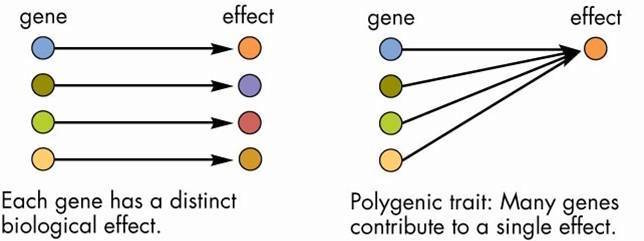
\includegraphics[width=2.1in]{stuff/polygenicA.jpg}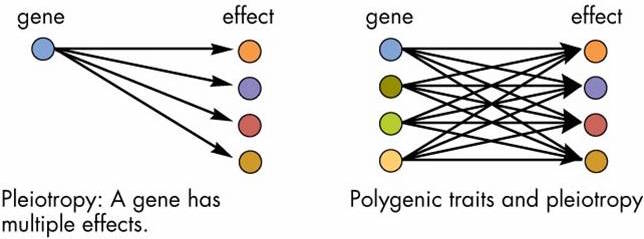
\includegraphics[width=2.1in]{stuff/polygenic.jpg} \\${}$\\


\begin{columns}
\begin{column}{.3\textwidth}

\begin{figure}
\tiny
\centering

$\left[\begin{array}{cccc}
\sigma_1^2 & 0 & \cdots & 0\\
0 & \sigma_2^2 &  \cdots & 0\\
\vdots & \vdots &  \ddots & \vdots \\
0 & 0 &  \cdots & \sigma_2^2\\
\end{array}\right]$\\${}$\\

\scriptsize
Experimental Design
\end{figure}

\end{column}
\begin{column}{.2\textwidth}
\large
$$f(Y|{\boldsymbol X})$$
\vspace*{-2em}
\begin{figure}[h!]
\centering
\scriptsize
Predictive Modeling
\end{figure}

\end{column}
\begin{column}{.3\textwidth}

\tiny

\vspace*{1.5em}

$\left[\begin{array}{cccc}
1^2 & r_{12} & \cdots &  r_{1p}\\
 r_{21} & 1^2 &  \cdots &  r_{2p}\\
\vdots & \vdots &  \ddots & \vdots \\
 r_{p1} &  r_{p2} &  \cdots & 1^2\\
\end{array}\right]$\\${}$\\

\scriptsize
$\quad\;$Correlated Features


\end{column}
\begin{column}{.15\textwidth}
\vspace*{-2em}
\begin{figure}[h!]
\large
PCA\\
FA\\
ICA\\
\end{figure}

\end{column}

\begin{column}{.1\textwidth}
\end{column}

\end{columns}


}



\frame
{
\frametitle{Objectives}

\begin{itemize}
\item Covariance Matrices Vs. Correlation Matrices 
\begin{itemize}
\item And what they do
\end{itemize}
\item Eigen-vectors/values of Correlation \& Covariance Matrices
\begin{itemize}
\item And what they do:
\item Proportion of Variance Explained
\begin{itemize}
\item Skree Plot
\end{itemize}
\item Directions
\item Projecting onto eigenvectors
\end{itemize}
\item Principal Components Analysis (PCA)
\begin{itemize}
\item Interpretation
\begin{itemize}
\item Biplots
\end{itemize}
\item Dimensionality Reduction
\item Visualization
\end{itemize}
\item Singular Value Decomposition (SVD)
\begin{itemize}
\item Same, but better than PCA?
\end{itemize}
\item Factor Analysis (FA)
\item Independent Component Analysis (ICA)
\end{itemize}
}



\frame
{
\frametitle{Sample Covariance Matrix}

\vspace{-1em}

\begin{columns}
\begin{column}{.25\textwidth}

 \huge $\quad\quad \quad {\boldsymbol X}_{n \times p}$:
\normalsize

\end{column}
\begin{column}{.75\textwidth}

\scriptsize

\begin{table}
\centering
\begin{tabular}{|r||l|l|l|l|}
\hline
Feature & $X_1$ & $X_2$ & $\cdots$ & $X_p$  \\  \hline \hline
n=1 &&&&\\  \hline
2 &&&& \\ \hline
$\vdots$ &&&& \\ \hline
n &&&& \\ \hline
\end{tabular}
\end{table}

\end{column}
\end{columns}

\vspace{-.5em}
\onslide<2->{
the sample \emph{covariance matrix} and \emph{correlation matrix}
capture observed feature covariances and correlations, respectively

\vspace{-.5em}
\scriptsize

\begin{columns}

\begin{column}{.05\textwidth}
\end{column}

\begin{column}{.45\textwidth}
\begin{table}
\scriptsize
\centering
\begin{tabular}{|r||l|l|l|l|}
\hline
$\mathbf{S_{p \times p}}$ & $X_1$ & $X_2$ & $\cdots$ & $X_p$ \\  \hline  \hline
$X_1$ & $\sigma_{11}^2$ & $\sigma_{12}^2$ && $\sigma_{1p}^2$ \\  \hline
$X_2$ &$\sigma_{21}^2$  &$\sigma_{22}^2$ && $\sigma_{2p}^2$ \\ \hline
$\vdots$ &&$\ddots$&& \\ \hline
$X_p$ &$\sigma_{p1}^2$ &$\sigma_{p2}^2$ && $\sigma_{pp}^2$ \\ \hline
\end{tabular}
\end{table}

\end{column}
\begin{column}{.5\textwidth}

\begin{table}
\centering
\begin{tabular}{|r||l|l|l|l|}
\hline
 $\mathbf{R_{p \times p}}$ & $X_1$ & $X_2$ & $\cdots$ & $X_p$ \\  \hline\hline
$X_1$ & $1$ & $r_{12}$ && $r_{1p}^{\;}$ \\  \hline
$X_2$ &$r_{21}$  &$1$ && $r_{2p}^{\;}$ \\ \hline
$\vdots$ &&$\ddots$&& \\ \hline
$X_p$ &$r_{p1}$ &$r_{p2}^{\;}$ && $1$ \\ \hline
\end{tabular}
\end{table}

\end{column}

\end{columns}
}
\normalsize

\color{gray}

\onslide<3->{

For a \textbf{centered} samples by features data matrix ($X_{ij} = X_{ij}^*- \bar X_{j}^*$) 

%\vspace{-.5em}


$\displaystyle \hat  S = \frac{1}{n-1}{\boldsymbol X}^T{\boldsymbol X} =  \frac{1}{n-1} \sum_{i=1}^n X_{i\cdot} X_{i\cdot}^T
\quad\quad\quad\quad\;\; \hat  R = \hat D_S^{-\frac{1}{2}}\hat S\hat D_S^{-\frac{1}{2}}$


\tiny
\vspace{.25em}
\hspace{.35in}$Cov(X_j,X_{j'}) =  \hat S_{jj'} =  \frac{1}{n-1}  \sum_{i=1}^n X_{ij} X_{ij'} $ \hspace{.45in} $D_S$ is the $p \times p$ matrix with same diagonal as $S$
}

}



\frame
{
\frametitle{Covariance versus Correlation}

\begin{figure}
\centering
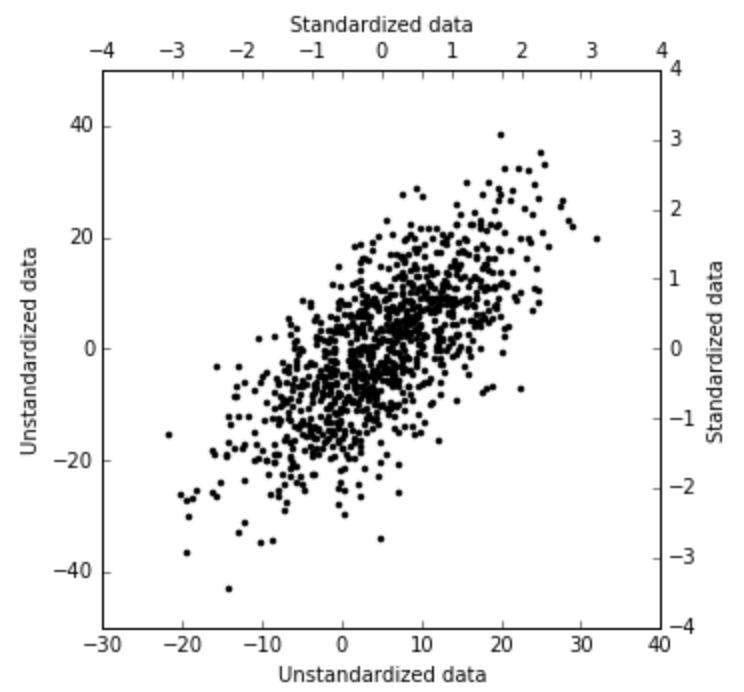
\includegraphics[width=3.5in]{stuff/covVcor.png}
\end{figure}

}


\frame
{
\frametitle{Sample Covariance (Correlation) Linear Transformation}

\begin{figure}
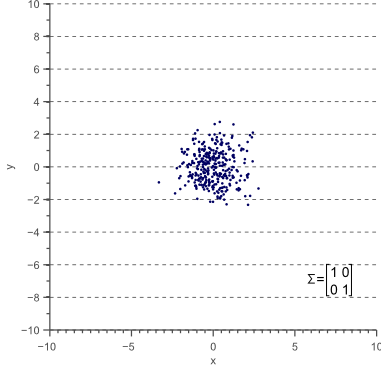
\includegraphics[width=2in]{stuff/whiteneddata.png}$\quad$
\raisebox{.5em}{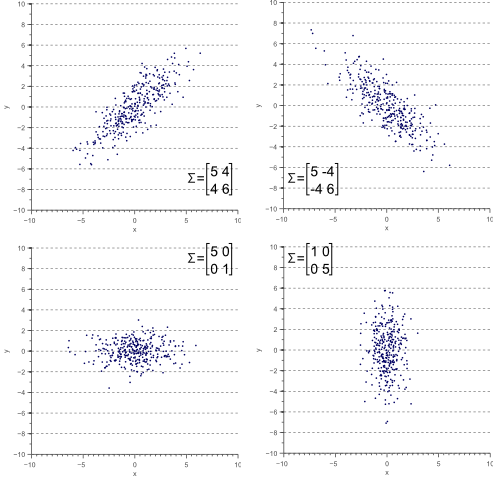
\includegraphics[width=1.925in]{stuff/covariances.png}}

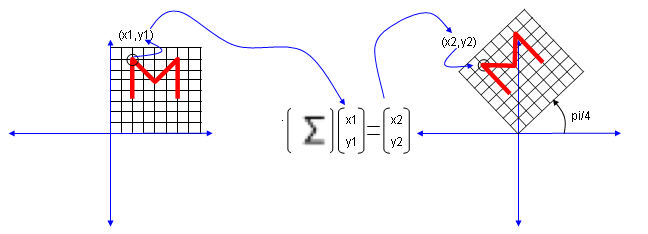
\includegraphics[width=4in]{stuff/EngMath_Matrix_Affin_Rotate.PNG}
\end{figure}




}


\frame
{
\frametitle{Eigenvectors and Eigenvalues}

The \emph{eigenvectors and eigenvalues} of a linear 
transformation $A_{p \times p}$ are orthonormal vectors $v$ and constants $\lambda$ satisfying
$$A v = \lambda v \quad \textcolor{gray}{\text{ as opposed to } \quad A w = w'}$$
\vspace{-1em}
$$
\left[\begin{array}{cc}2&0\\0&1\end{array}\right] \left[\begin{array}{cc}1\\0\end{array}\right] = 2\left[\begin{array}{cc}1\\0\end{array}\right] 
\quad\quad
\textcolor{gray}{\left[\begin{array}{cc}2&0\\0&1\end{array}\right] \left[\begin{array}{cc}\frac{1}{\sqrt{2}}\\\frac{1}{\sqrt{2}}\end{array}\right] = \left[\begin{array}{cc}\frac{2}{\sqrt{2}}\\\frac{1}{\sqrt{2}}\end{array}\right]} 
$$

\color{gray}

\vspace{-.5em}

\onslide<2->{
\begin{figure}
\centering
\footnotesize
The covariance (correlation) matrix correlates uncorrelated variables

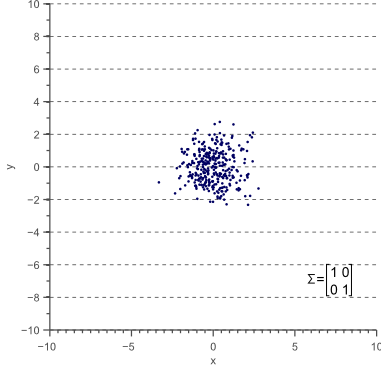
\includegraphics[width=.75in]{stuff/whiteneddata.png}
\raisebox{0em}{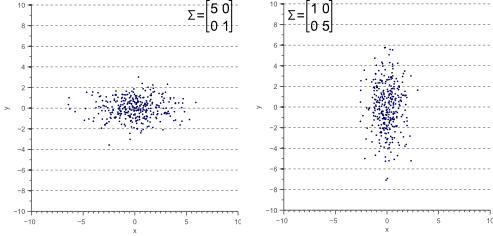
\includegraphics[width=1.5in]{stuff/covariances_b.png}}
\hspace{-.25em}\raisebox{0em}{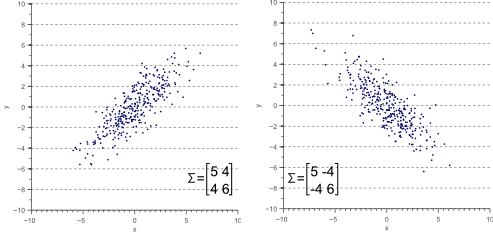
\includegraphics[width=1.5in]{stuff/covariances_a.png}}$\;\;\;$
\end{figure}
}

\vspace{-.5em}

\color{white}
\onslide<2->{

\underline{The \emph{eigenvectors} of the covariance (correlation) matrix turn out to}
\underline{ be unit vectors
$v_j$  sequentially maximizing the variance of \emph{scores}}
\underline{$z_{ij} = v_j^T X_{i\cdot}$ 
that are sequentially uncorrelated with previous \emph{scores}.}

%\vspace{.5em}

\textcolor{white}{I.e. for each $j$, $v_j$ solve $\underset{v_j}{argmax}  \sum_{j'=1}^jVar(z_{ij'}) = \sum_{j'=1}^j\lambda_{j'}$ 
such that $Cov(z_{ij}, z_{ij'})=0$  for $j'<j$, with  $\lambda_j$ the eigenvalue of $v_j$. }
}
}


\frame
{
\frametitle{Eigenvectors and Eigenvalues}

The \emph{eigenvectors and eigenvalues} of a linear 
transformation $A_{p \times p}$ are orthonormal vectors $v$ and constants $\lambda$ satisfying
$$A v = \lambda v \quad \textcolor{gray}{\text{ as opposed to } \quad A w = w'}$$
\vspace{-1em}
$$
\left[\begin{array}{cc}2&0\\0&1\end{array}\right] \left[\begin{array}{cc}1\\0\end{array}\right] = 2\left[\begin{array}{cc}1\\0\end{array}\right] 
\quad\quad
\textcolor{gray}{\left[\begin{array}{cc}2&0\\0&1\end{array}\right] \left[\begin{array}{cc}\frac{1}{\sqrt{2}}\\\frac{1}{\sqrt{2}}\end{array}\right] = \left[\begin{array}{cc}\frac{2}{\sqrt{2}}\\\frac{1}{\sqrt{2}}\end{array}\right]} 
$$

\color{gray}

\vspace{-.5em}

\onslide<1->{
\begin{figure}
\centering
\footnotesize
The covariance (correlation) matrix correlates uncorrelated variables

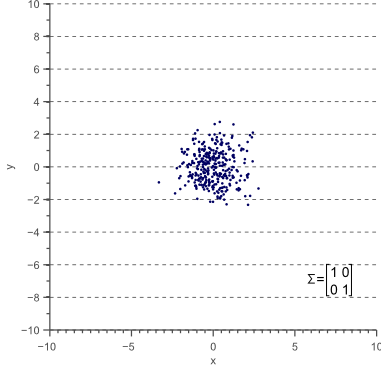
\includegraphics[width=.75in]{stuff/whiteneddata.png}
\raisebox{0em}{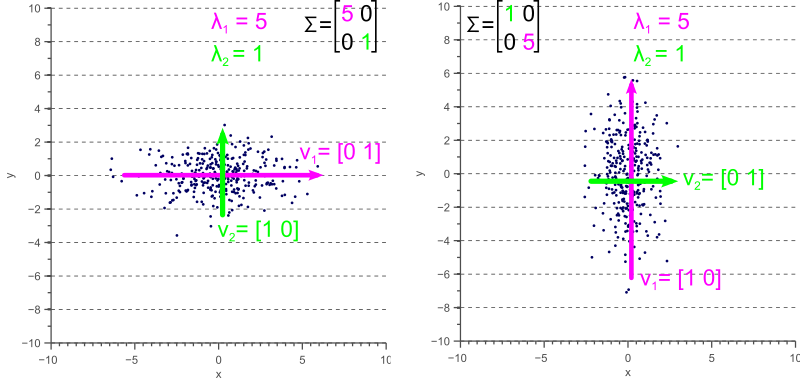
\includegraphics[width=1.5in]{stuff/eigenvectors.png}}
\hspace{-.25em}\raisebox{0em}{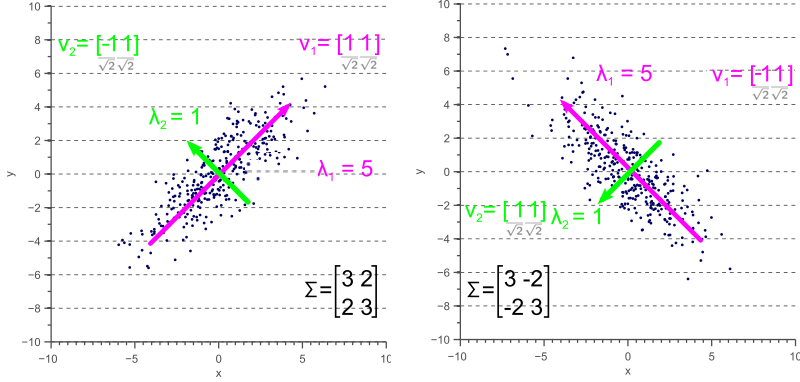
\includegraphics[width=1.5in]{stuff/eigenvectors_covariance.png}}$\;\;\;$
\end{figure}
}

\vspace{-.5em}

\color{black}
\onslide<1->{

\underline{The \emph{eigenvectors} of the covariance (correlation) matrix turn out to}
\underline{be unit vectors
$v_j$  sequentially maximizing the variance of \emph{scores}} 
\underline{$z_{ij} = v_j^T X_{i\cdot}$ 
that are sequentially uncorrelated with previous \emph{scores}.}

%\vspace{.5em}

\textcolor{gray}{I.e. for each $j$, $v_j$ solve $\underset{v_j}{argmax}  \sum_{j'=1}^jVar(z_{ij'}) = \sum_{j'=1}^j\lambda_{j'}$ 
such that $Cov(z_{ij}, z_{ij'})=0$  for $j'<j$, with  $\lambda_j$ the eigenvalue of $v_j$. }
}
}



\frame
{
\frametitle{Proportion of Variation Explained}

\color{gray}
Since our eigenvalues are orthonormal, i.e., 
\vspace{-.75em}

$$\sum_{k=1}^p v_{kj}^2 = 1 \text{ and } v_j^Tv_{j'} = 0 \text{ for } j \not = j' \; \text{we have that}$$
\vspace{-.5em}
$$\sum_{j=1}^p \underset{i}{Var}(X_{ij}) = \sum_{j=1}^p \underset{i}{Var}(v_{j}^T X_{i\cdot}) = \sum_{j=1}^p \underset{i}{Var}(z_{ij}) = \sum_{j=1}^p \lambda_{j}$$

\color{black}
I.e., data variance cay be partitioned between eigenvector directions\\




\begin{columns}
\begin{column}{.525\textwidth}

\onslide<1->{

\vspace{-.7in}
\begin{figure}
\centering
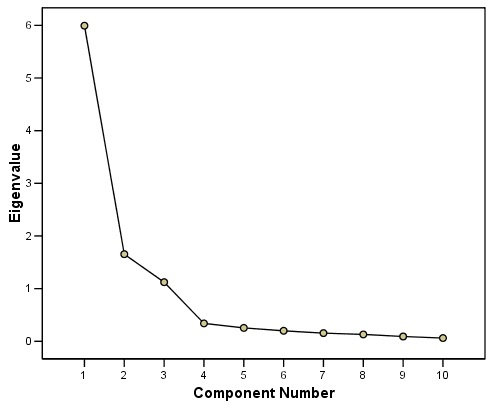
\includegraphics[width=2.35in]{stuff/screep.jpg}

\vspace{-1.75in}
$\quad\quad\quad$ The proportion of variance\\
$\quad\quad\quad$  attributable to the  $j$th \\
$\quad\quad\quad$ eigenvector direction is  
$$\quad\quad\quad\frac{\lambda_{j}}{\sum_{j'=1}^p \lambda_{j'}}$$

\end{figure}
}

\end{column}
\begin{column}{.5\textwidth}
\vspace{.1in}

\onslide<1->{
\hspace{-.05in}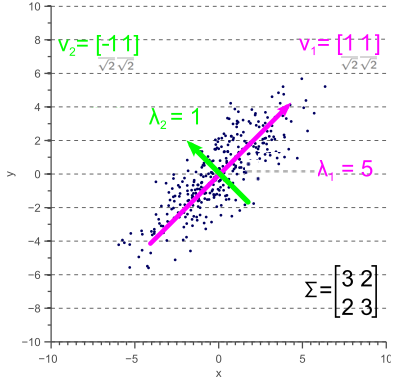
\includegraphics[width=2in]{stuff/eigenvectors_covariance_small.png}
}
\end{column}
\end{columns}


${}$\\${}$\\${}$\\${}$\\${}$\\${}$\\${}$\\

}



\frame
{
 \frametitle{\emph{Biasing} the ``Proportion of Variance Explained'' \emph{Direction}}

The eigenvalues point towards the most correlated axes, e.g.

\tiny 
$$
\left[
\begin{array}{cccc}
1 & 0.9 & 0.1 &  0.1\\
0.9 & 1 & 0.1 &  0.1\\
 0.1 &  0.1 & 1 & 0.9 \\
 0.1 &  0.1 & 0.9 & 1 \\
\end{array}
\right]
\quad v_1 = 
1/\sqrt{\frac{1}{4}}\left[
\begin{array}{c}
1 \\
1 \\
1  \\
1  \\
\end{array}
\right]
\quad  v_2 = 
1/\sqrt{\frac{1}{4}}\left[
\begin{array}{c}
-1 \\
-1 \\
\textcolor{white}{-}1  \\
\textcolor{white}{-}1  \\
\end{array}
\right]
$$

$$
\left[
\begin{array}{ccc}
1 & .6 & .5 \\
.6 & 1 & .4 \\
.5 &  .4 & 1  \\
\end{array}
\right]
\quad  v_1 = 
\left[
\begin{array}{c}
0.61\\
0.58\\
0.54
\end{array}
\right]
$$

$\;$

$\;$

\normalsize

\onslide<2->{
The eigenvalues further point towards high variance axes, e.g.


\begin{figure}
\centering
$\quad$\raisebox{.5em}{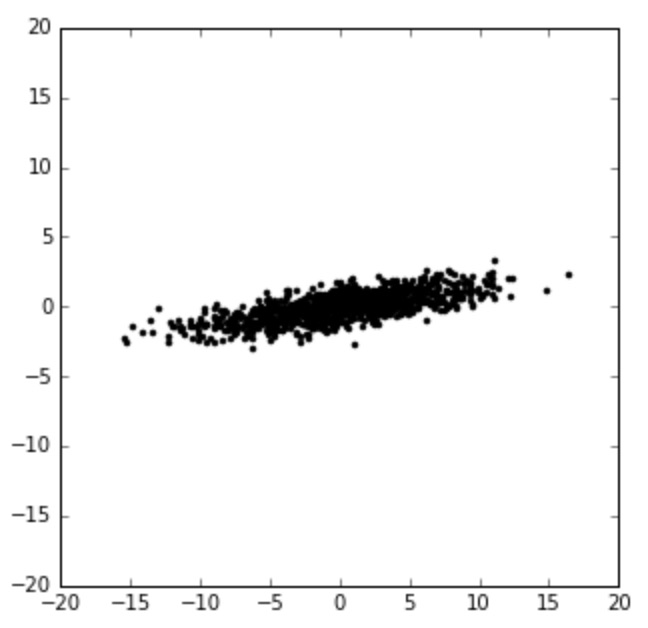
\includegraphics[width=1.5in]{stuff/normalize.jpg}}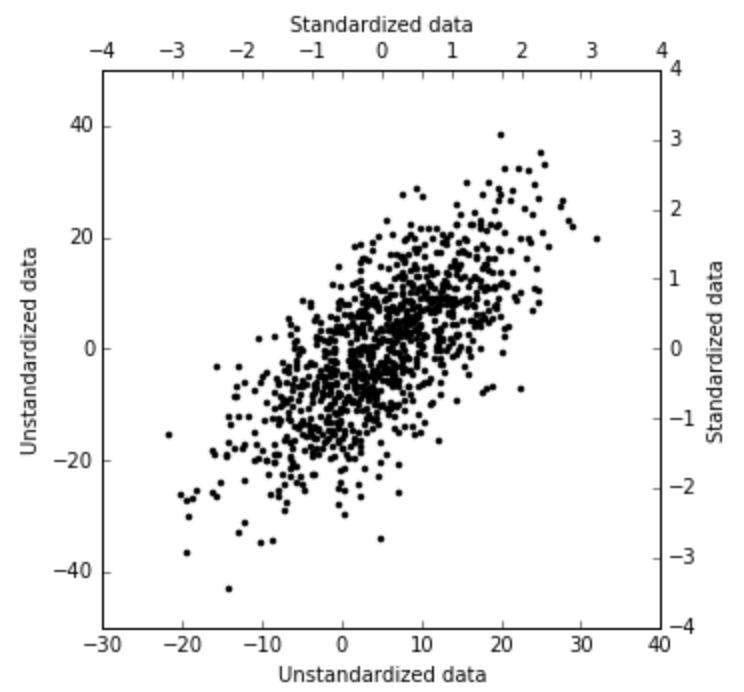
\includegraphics[width=1.75in]{stuff/covVcor.png}
\end{figure}}

\onslide<3->{
\vspace{-1em}
\textcolor{gray}{When is $\sum_{j=1}^p \lambda_{j} = p$?}}

}







\frame
{
 \frametitle{Mapping onto the directions of  \emph{``Greatest Variation''}}
 
 \hspace{.5em}
 
 The orthogonally projection of $X_i$ onto $v_j$ is 
 $$z_{ij} = \frac{v_j}{||v_j||} \cdot X_i$$
 
For unit \emph{eigenvectors} $v_j$, this is simply the dot product
 $$z_{ij} = v_j \cdot X_i$$

\vspace{-2.5em}

\begin{figure}
\hspace*{-2em}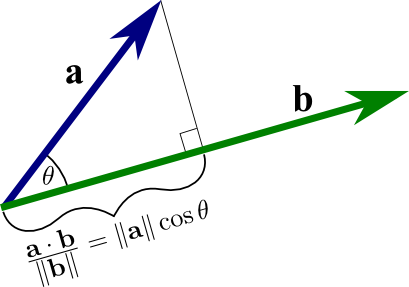
\includegraphics[width=2in, angle=21]{stuff/dot_product_projection.png}
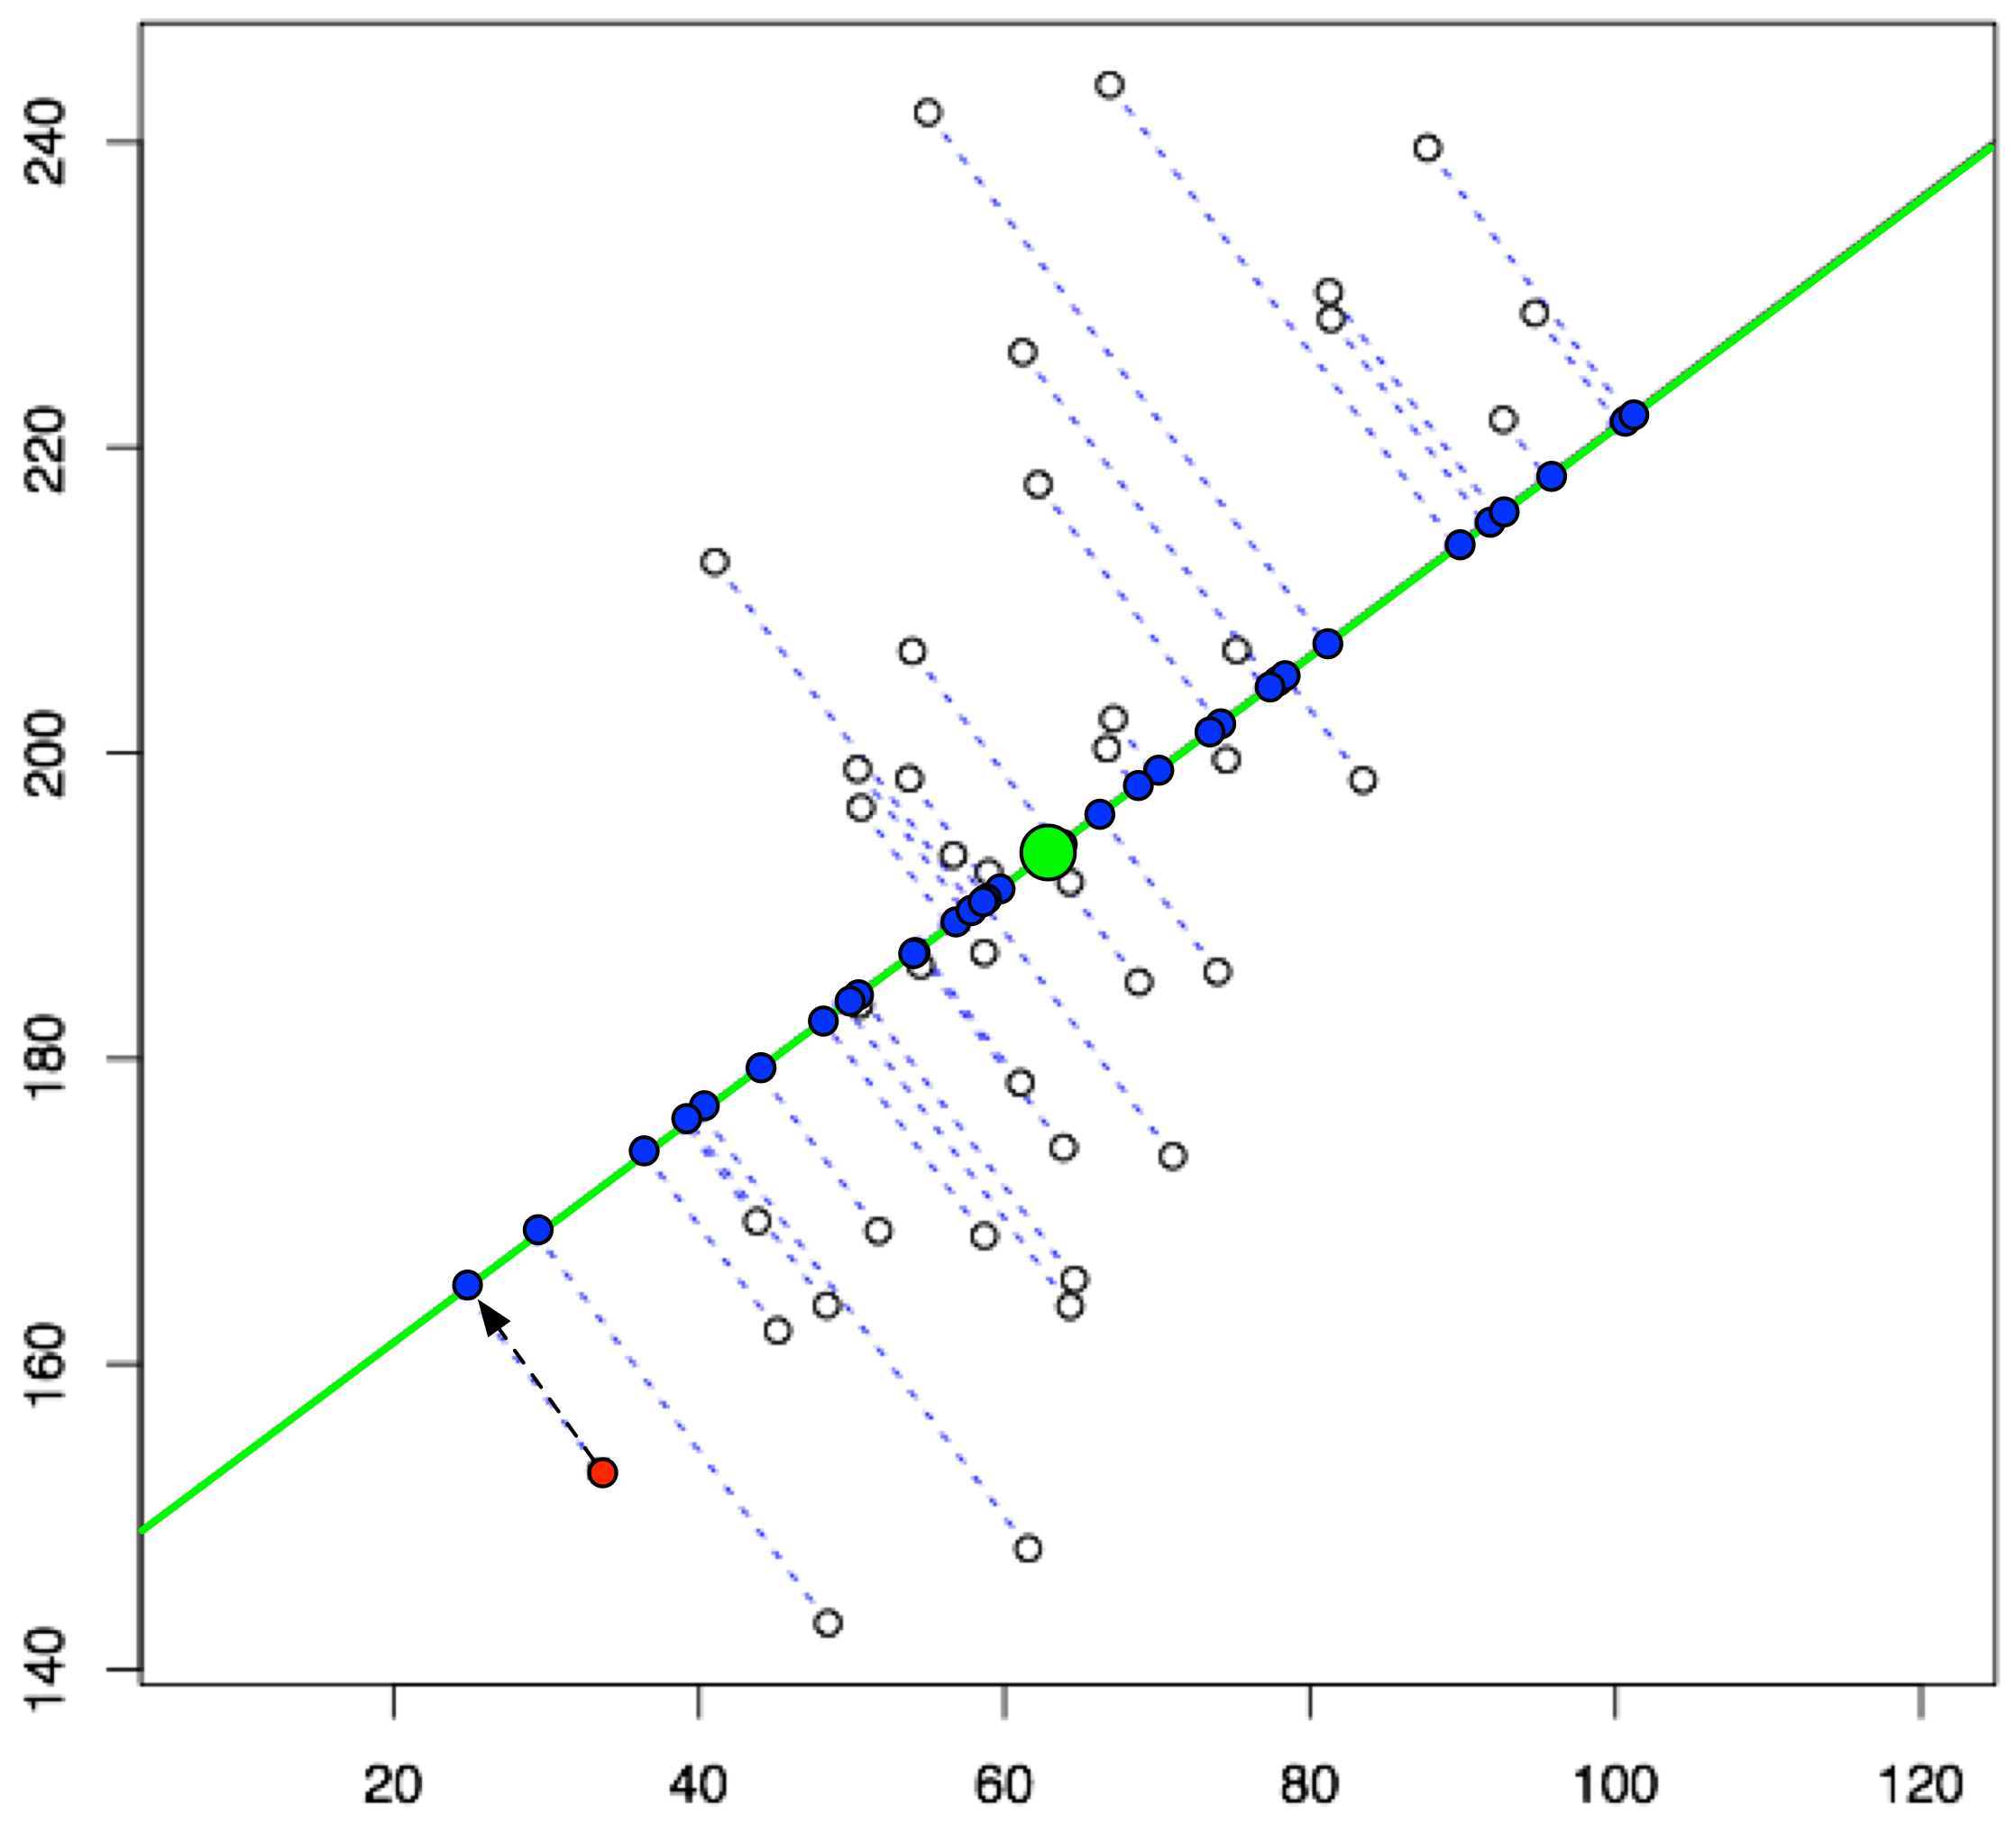
\includegraphics[width=2in]{stuff/pca_figure1.jpg}
\end{figure}
 
}


\frame
{
\frametitle{Principal Components Analysis (PCA)}


\begin{itemize}
\item PCA projects ${\boldsymbol X}$ onto the ${\boldsymbol X}$'s covariance matrix eigenvectors
\item An eigenvector projection is called a \underline{principal component (PC)} 
\item \textcolor{gray}{The $1^{st}$ \emph{PC}  is the projection onto the eigenvector with the \emph{largest eigenvalue},
the  $2^{nd}$ \emph{PC} is the projection onto the eigenvector with the \emph{second largest eigenvalue}, etc.}

\item<2-> The \emph{Principal Components} ${\boldsymbol z}$ are an orthogonal rotation of ${\boldsymbol X}$
\end{itemize}

\onslide<2->{ 
\vspace{-.75em}
\begin{table}
\centering
\begin{tabular}{|r||l|l|l|l|}
\hline
Feature & $X_1$ & $X_2$ & $\cdots$ & $X_p$  \\  \hline \hline
n=1 &&&&\\  \hline
2 &&&& \\ \hline
$\vdots$ &&&& \\ \hline
n &&&& \\ \hline
\end{tabular}
$\longrightarrow$
\begin{tabular}{|r||l|l|l|l|}
\hline
PC & $z_1$ & $z_2$ & $\cdots$ & $z_p$  \\  \hline \hline
n=1 &&&&\\  \hline
2 &&&& \\ \hline
$\vdots$ &&&& \\ \hline
n &&&& \\ \hline
\end{tabular}
\end{table}}

\vspace{-.75em}
\begin{itemize}
\item<3->  PCA routinely centers and scales $X_{\cdot j}$ in order to capture correlation between features rather than feature scales
\end{itemize}

}


\frame
{
 \frametitle{PCA: transforming into uncorrelated features...}

$\quad\quad$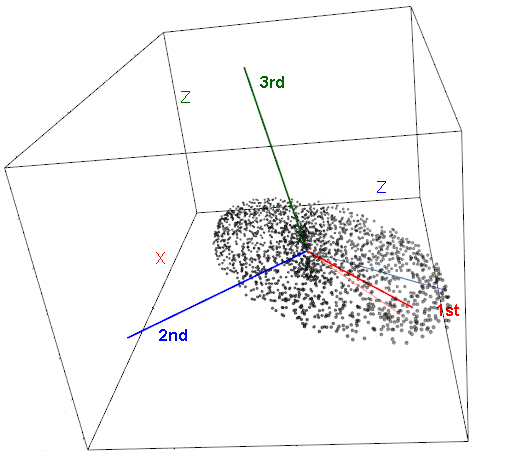
\includegraphics[width=3.25in, angle=-5]{stuff/WgiUk.png}

}


\frame
{
 \frametitle{Biplots}

\begin{itemize}
\item Vector: $k^{th}$ versus $k'^{th}$ eigenvector's $j^{th}$ feature loading: $$v_{kj} \text{ versus }v_{k'j}$$
\item Point: observation $i$'s $j^{th}$ versus $j'^{th}$  PC scores: $$z_{ji} = v_{j}'X_{i} \text{ versus } z_{j'i} = v_{j'}'X_{i}$$
\end{itemize}

\vspace{-3em}

\begin{columns}
\begin{column}{.01\textwidth}
\end{column}
\begin{column}{.4\textwidth}
\begin{figure}
\centering
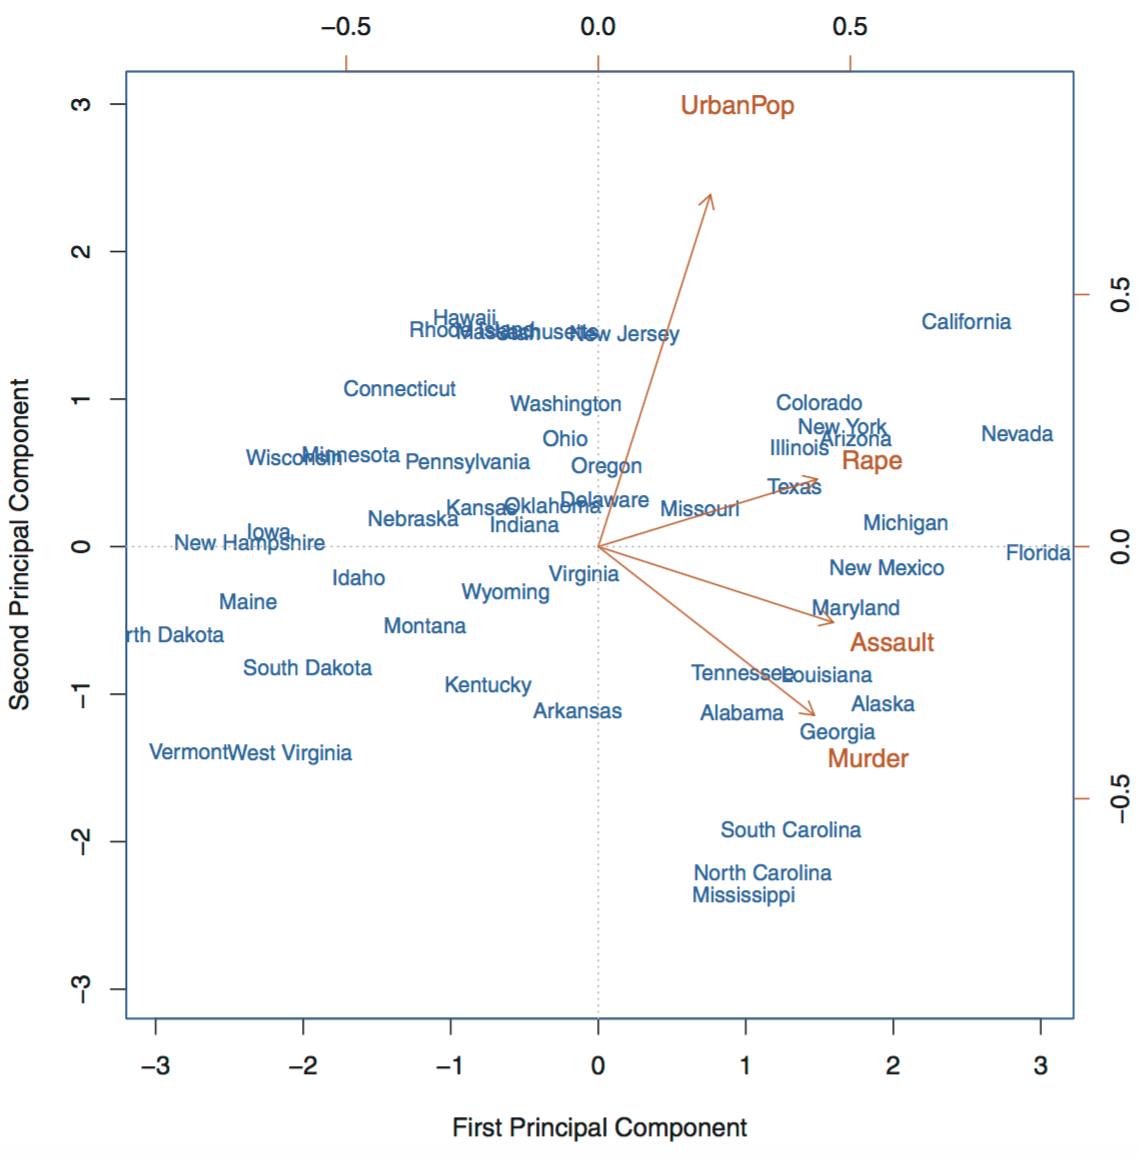
\includegraphics[width=2.25in]{stuff/biplot.png}
\end{figure}

\end{column}
\begin{column}{.4\textwidth}

\begin{figure}

\vspace{.4em}

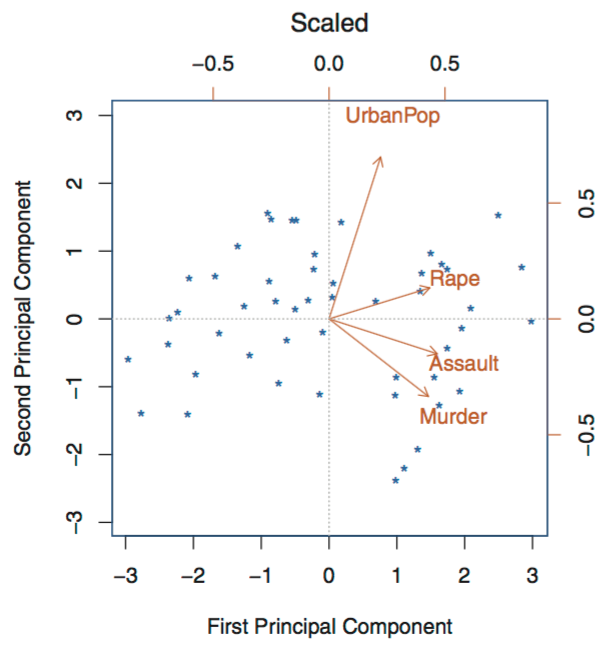
\includegraphics[width=1.03in]{stuff/biplot2b.png}

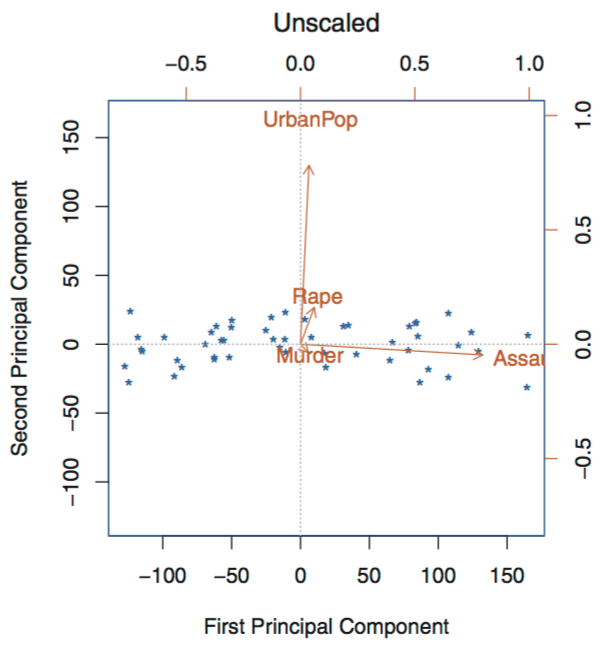
\includegraphics[width=1.03in]{stuff/biplot2.png}
\end{figure}

\end{column}

\end{columns}

}


\frame
{
 \frametitle{Dimensionality \textcolor{gray}{Reduction?}}

\onslide<3->{
How does e.g. KNN feel about this many dimensions? \textcolor{gray}{Curse of...}\\${}$\\
}

\only<2->{\raisebox{.15em}{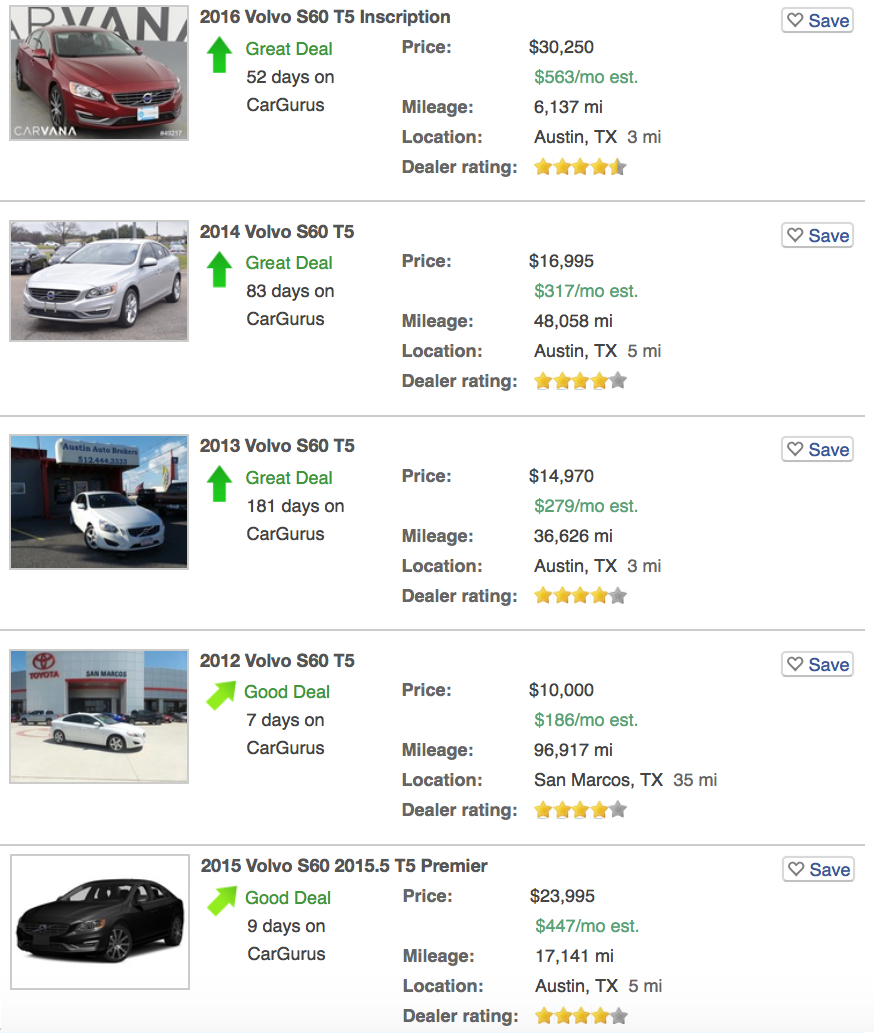
\includegraphics[width=2in]{stuff/carsB.jpg}}
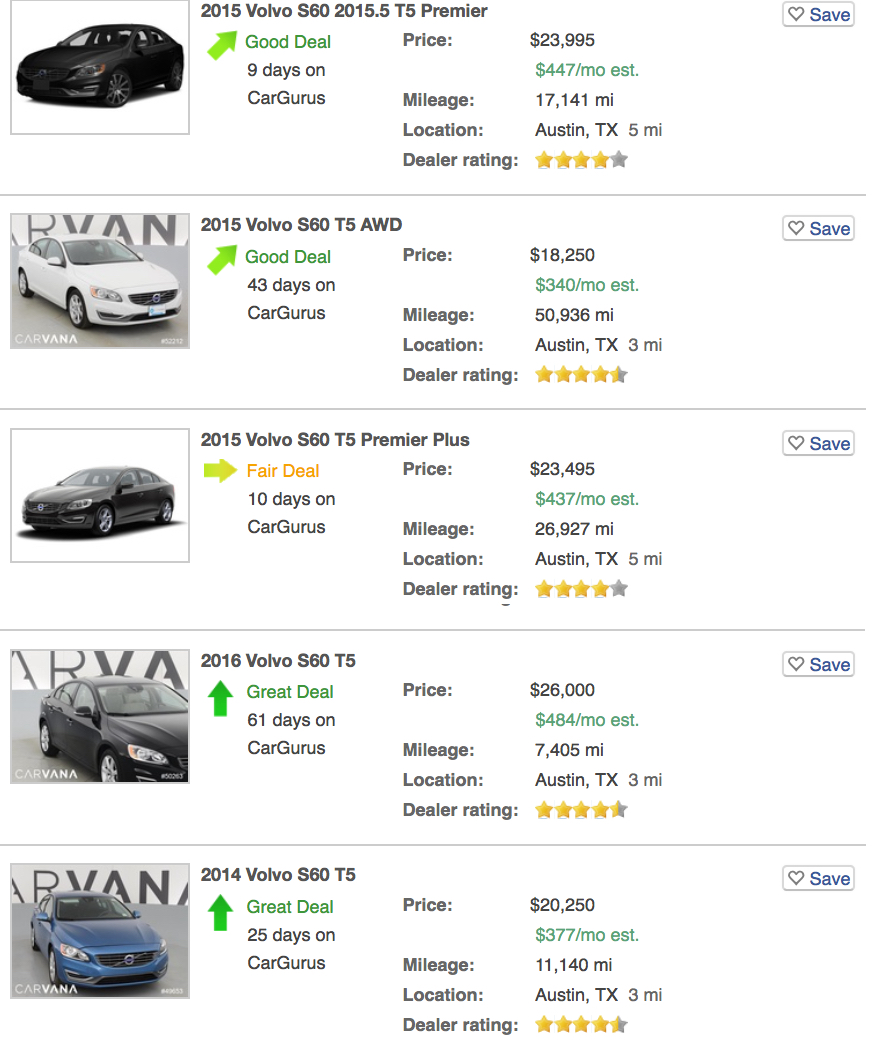
\includegraphics[width=1.99in]{stuff/carsC.jpg}}

\only<1>{\raisebox{.15em}{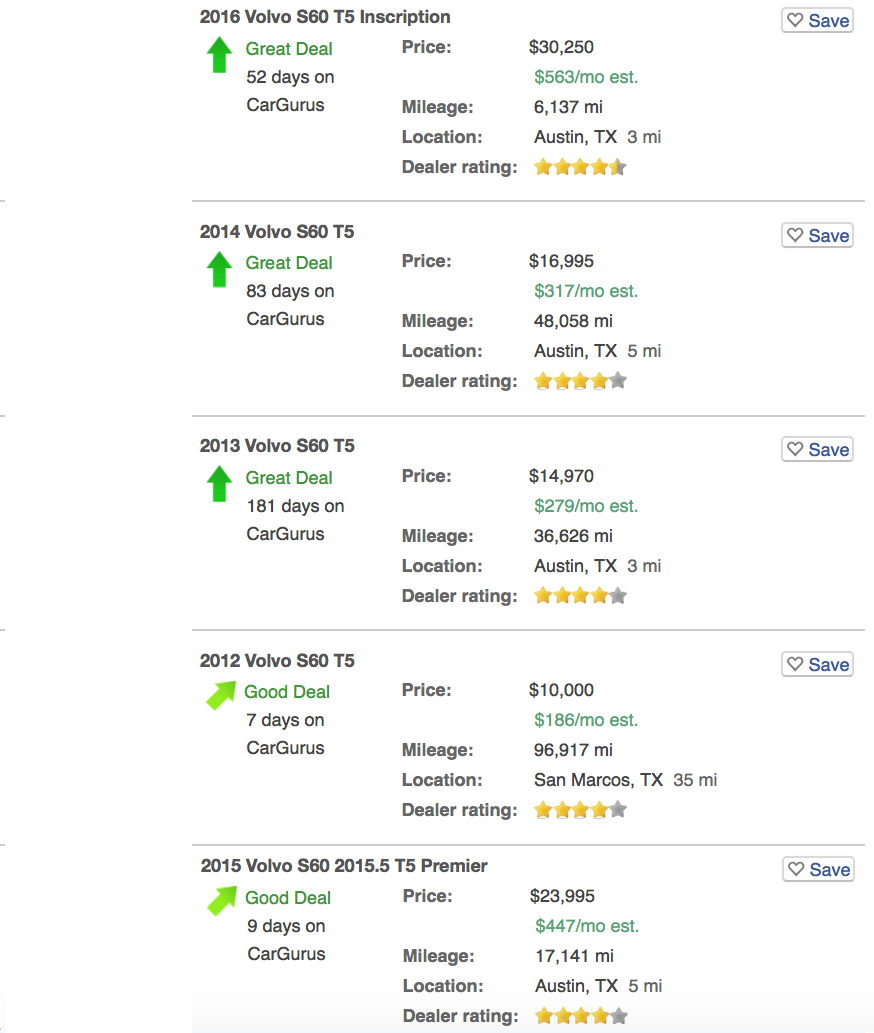
\includegraphics[width=2in]{stuff/carsBb.jpg}}
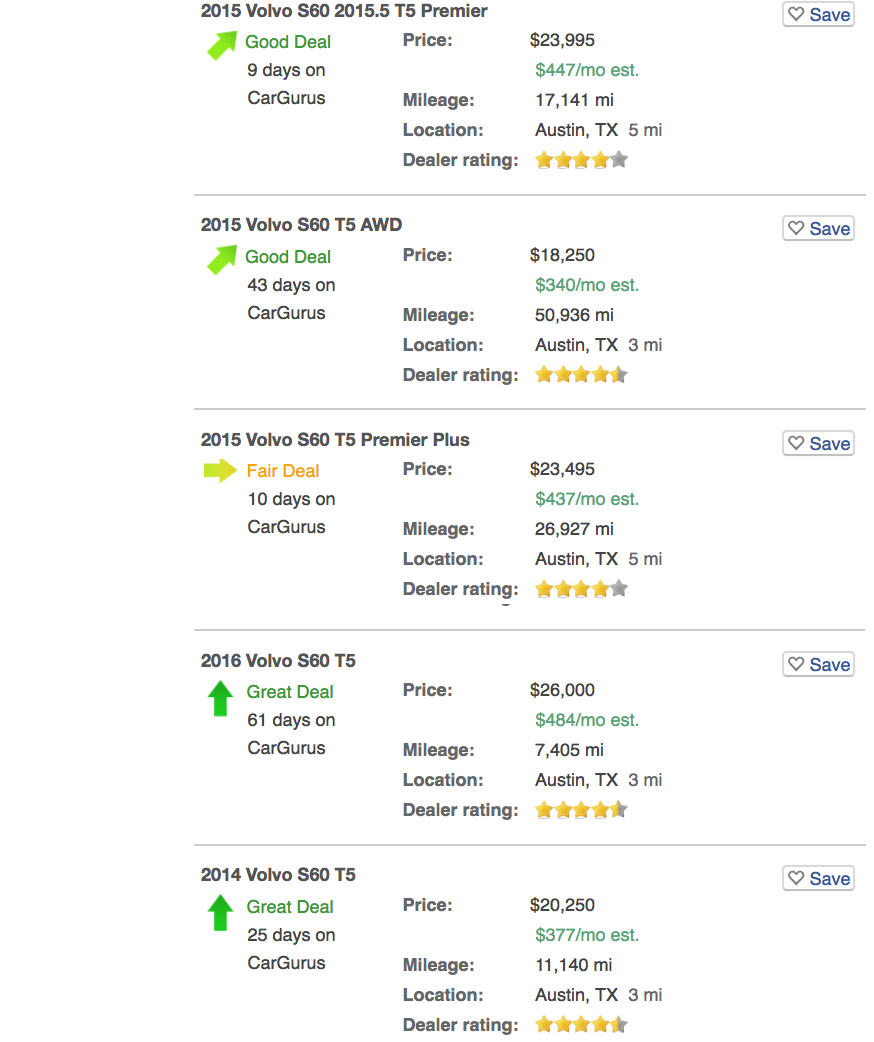
\includegraphics[width=1.99in]{stuff/carsCb.jpg}}


}



\frame
{
 \frametitle{Dimensionality Reduction}


 

 \vspace{-1.5em}
 
\begin{columns}
\begin{column}{.02\textwidth}
\end{column}
\begin{column}{.34\textwidth}

 %np.linalg.eig  
 %Ddimension\\ 
 %reduction:  
 $$\quad \underset{p\times1}{X_{i}} \approx \sum_{j=1}^{q<p} \underset{p\times1}{v_{j}} z_{ij} $$\\${}$\\${}$\\${}$\\

\end{column}
\begin{column}{.5\textwidth} 
 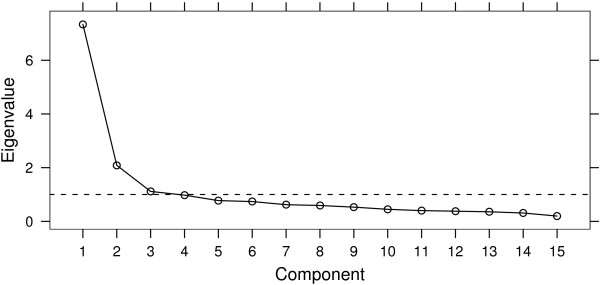
\includegraphics[width=1.7in]{stuff/screeplot.jpg} 
\end{column}
 \end{columns}
 
 \vspace{-2.5em}

\onslide<2->{
 \begin{figure}
 \centering
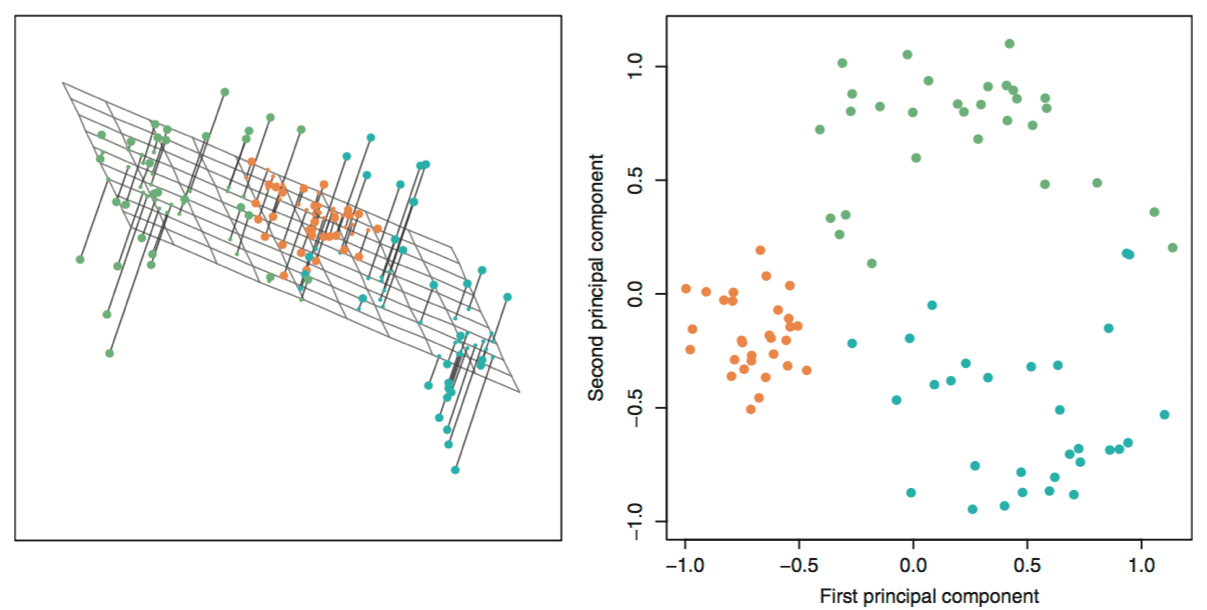
\includegraphics[width=3.5in]{stuff/pca2.png} 

\onslide<3->{
\textcolor{black}{Compresses data into uncorrelated variation \& maybe drops noise\\
 (\underline{Feature Engineering?}) (\underline{Curse of Dimensionality?})}
}

\color{gray}
\footnotesize
\vspace{.5em}
\onslide<4->{
The number of \emph{nonzero} $\lambda_{j}$'s equals the rank of the covariance \\
matrix ${\boldsymbol X}^T{\boldsymbol X}$ which itself equals the rank of the data matrix ${\boldsymbol X}$
}

\end{figure}

}
}


\frame
{
 \frametitle{Dimensionality Reduction \textcolor{gray}{Examples}}

\begin{columns}
\begin{column}{.1\textwidth}
\end{column}
\begin{column}{.35\textwidth}
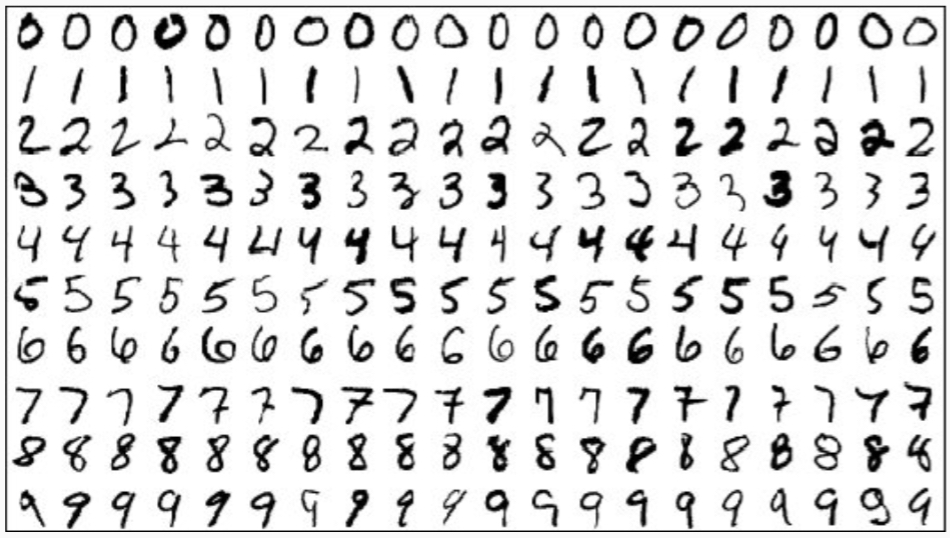
\includegraphics[width=1.5in]{stuff/mnist1.jpg}


\onslide<2->{\hspace*{-.1in}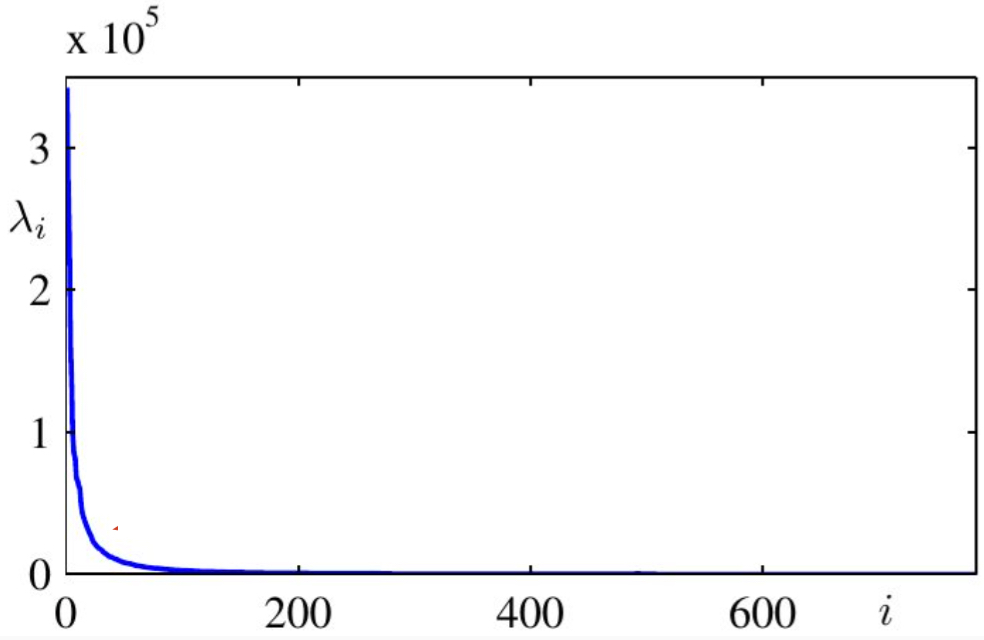
\includegraphics[width=1.6in]{stuff/mnist2.jpg}}

\onslide<3->{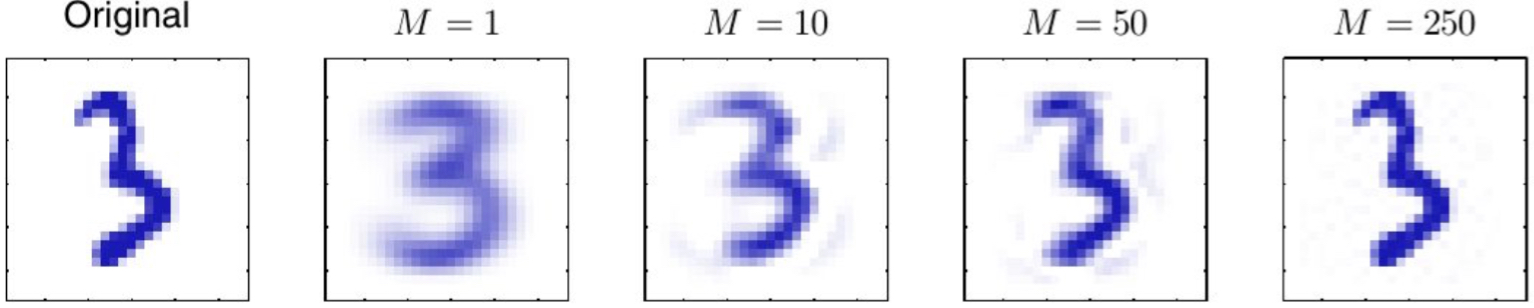
\includegraphics[width=1.5in]{stuff/mnist3.jpg}}

\onslide<4->{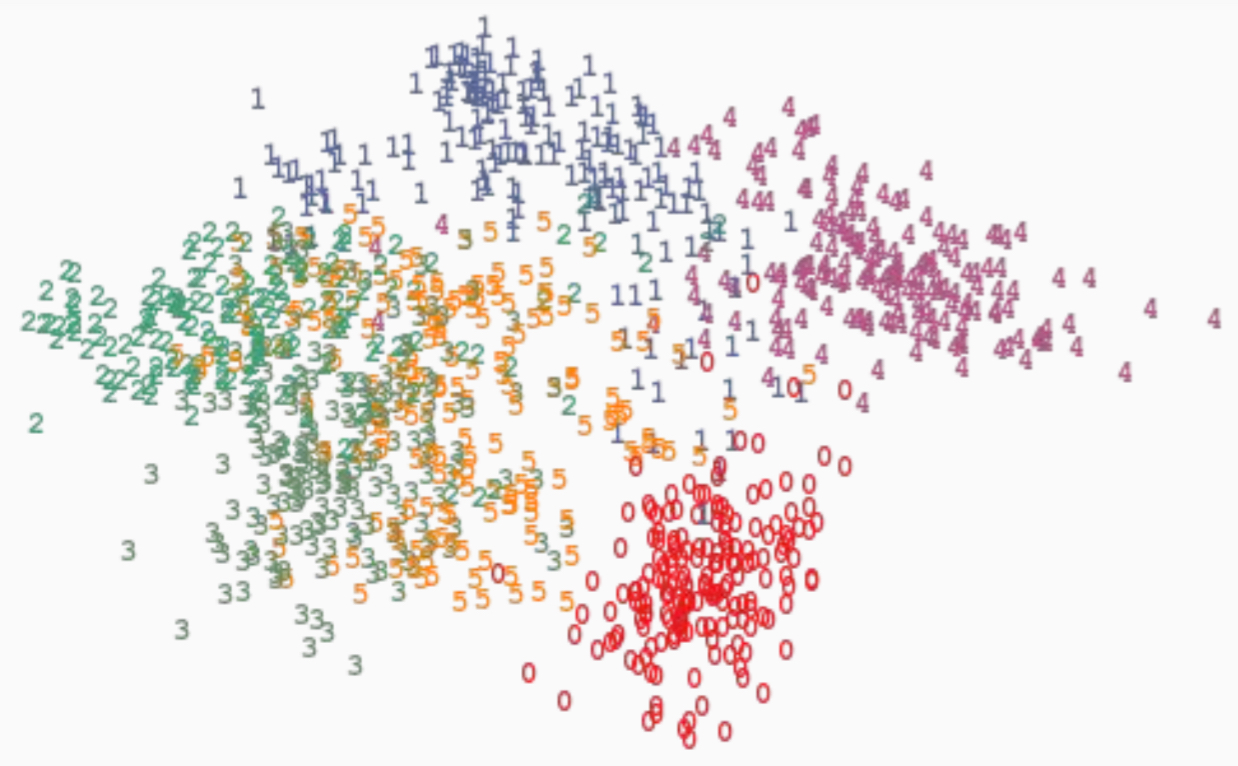
\includegraphics[width=1.5in]{stuff/mnist4.jpg}}
\end{column}
\begin{column}{.1\textwidth}
\end{column}
\begin{column}{.65\textwidth}

\onslide<5->{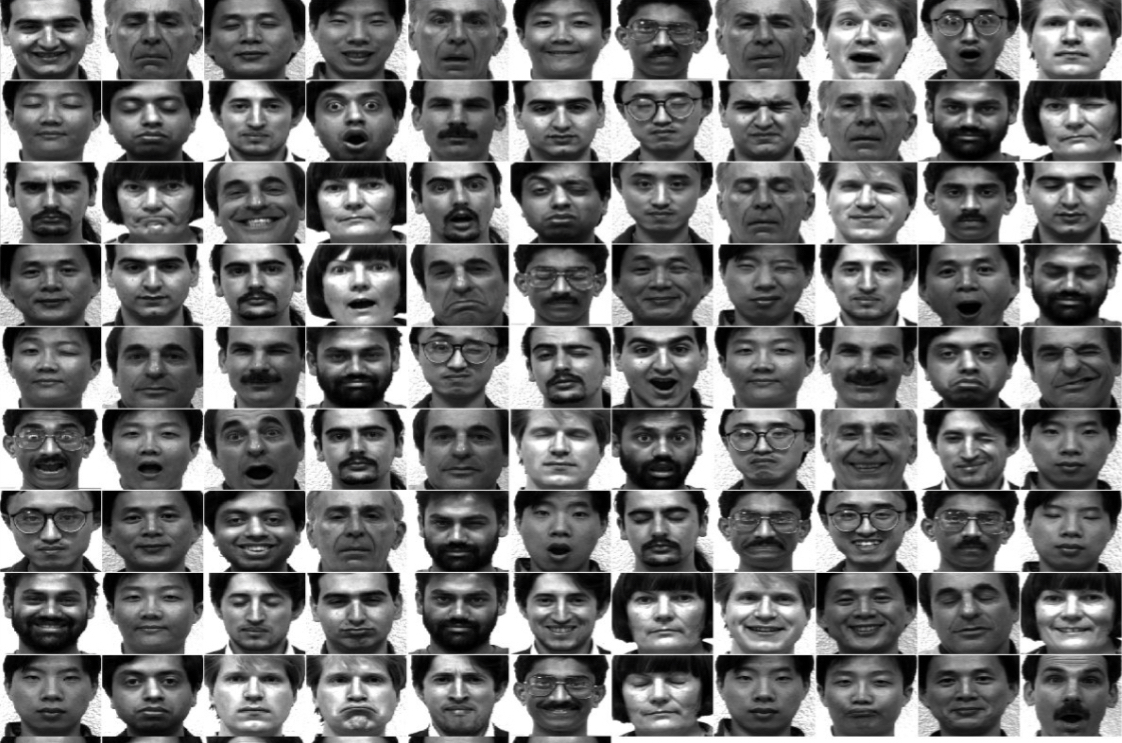
\includegraphics[width=2.22in]{stuff/faces1.jpg}}

\onslide<6->{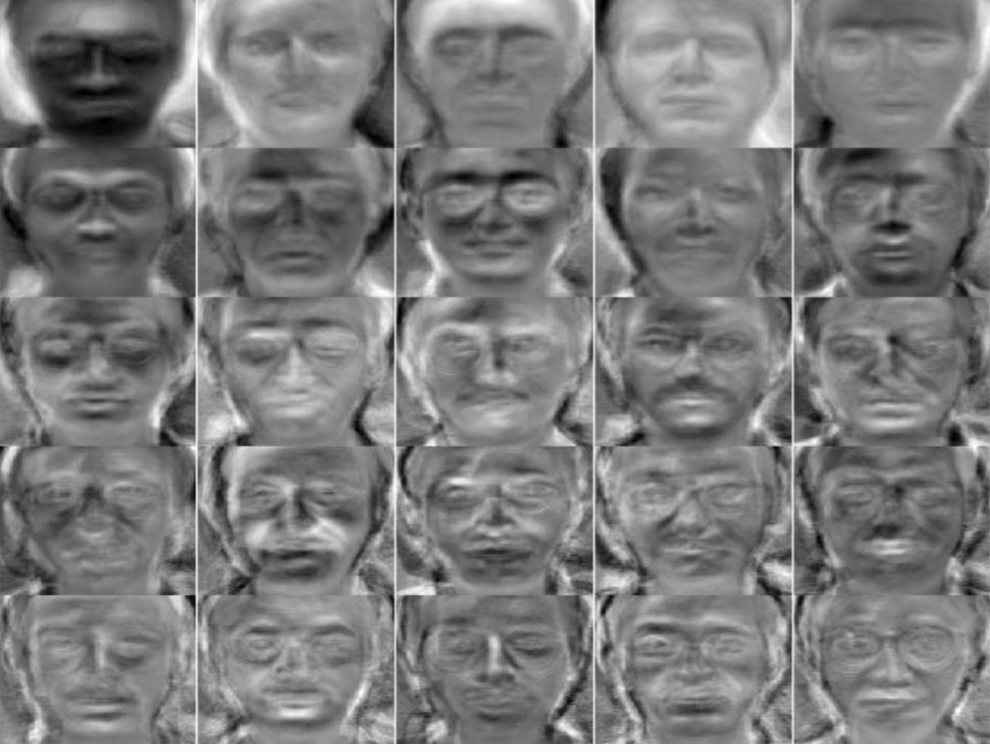
\includegraphics[width=2.22in]{stuff/faces2.jpg}}

\end{column}
\end{columns}



}


\frame
{
 \frametitle{Visualization (for EDA purposes)}

 \begin{figure}
 \centering
\rotatebox{90}{\hspace{1.25in}$2^{nd} PC$}\;\;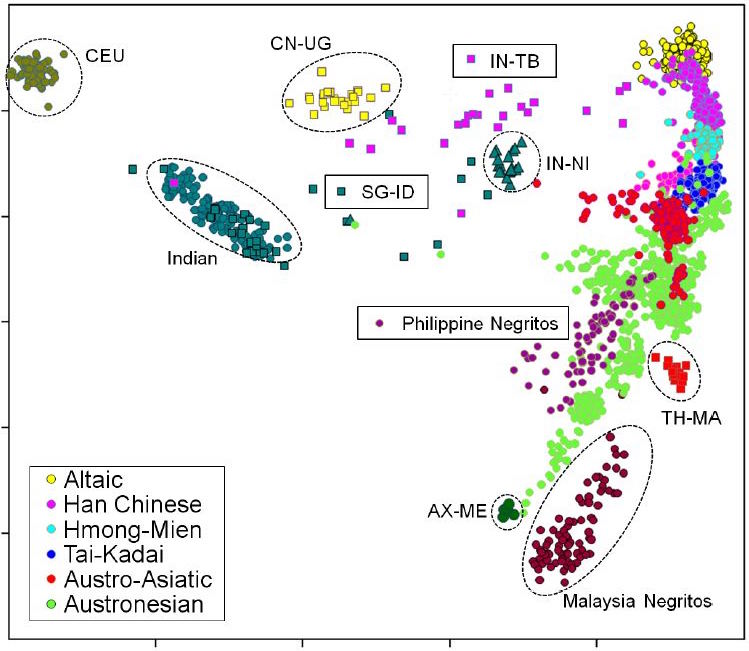
\includegraphics[width=3.25in]{stuff/dna_pca.jpg}

$\quad 1^{st} PC$
\end{figure}

}



\frame
{
 \frametitle{How else could we do dimension reduction?}

\begin{columns}
\begin{column}{.4\textwidth}

\begin{itemize}
\item<2-> Stepwise Selection
\item[]
\item[]
\item<3-> Lasso
\item[]
\item[]
\item[]
\item[]
\item<4-> Neural Networks
\item[]
\item[]
\item[]
\item[]<7-> \textcolor{gray}{It's fun to stay at the}
\item<7-> PCA\textcolor{gray}{, eh?}  
\end{itemize}

\end{column}
\begin{column}{.65\textwidth}

\only<2>{\vspace{-1.15in}}
\only<3>{\vspace{-1.15in}}
\only<4>{\vspace{-.085in}}
\only<5>{\vspace{.15in}}
\only<6>{\vspace{-.1in}}
\only<7>{\vspace{-.1in}}
\onslide<2->{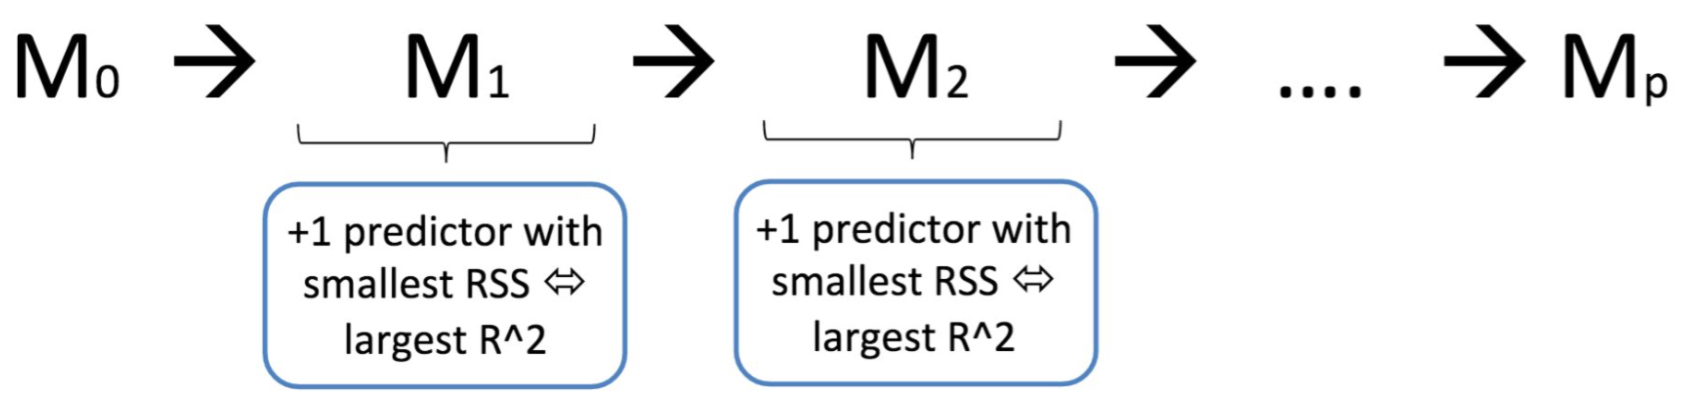
\includegraphics[width=2.25in]{stuff/stepWIZE.jpg}}${}$\\${}$\\


\onslide<3->{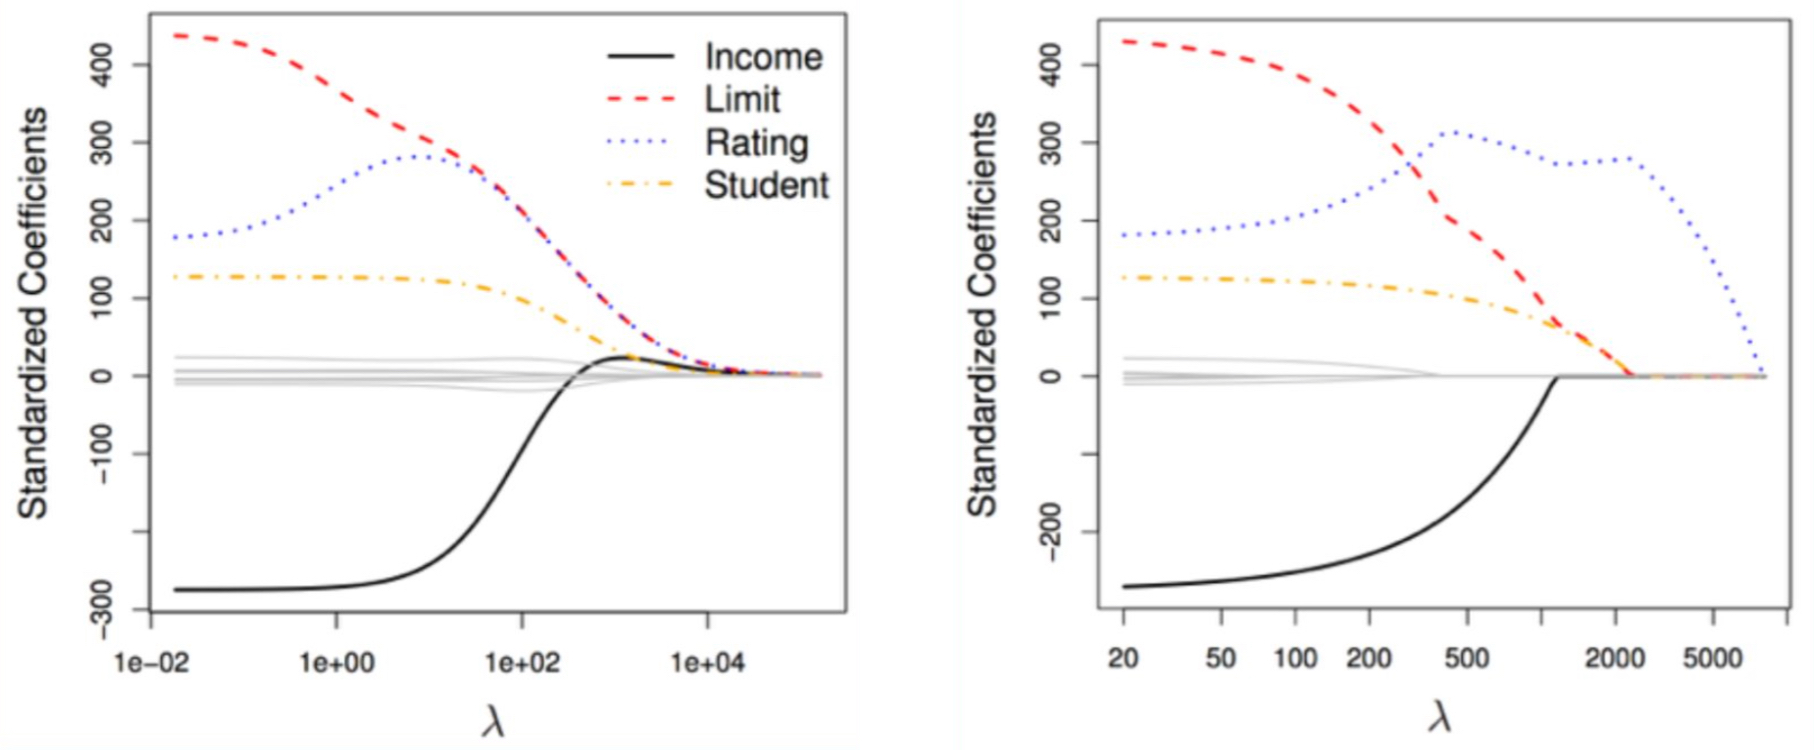
\includegraphics[width=2.25in]{stuff/ridge_pca.jpg}}${}$\\${}$\\

\only<4>{$\quad$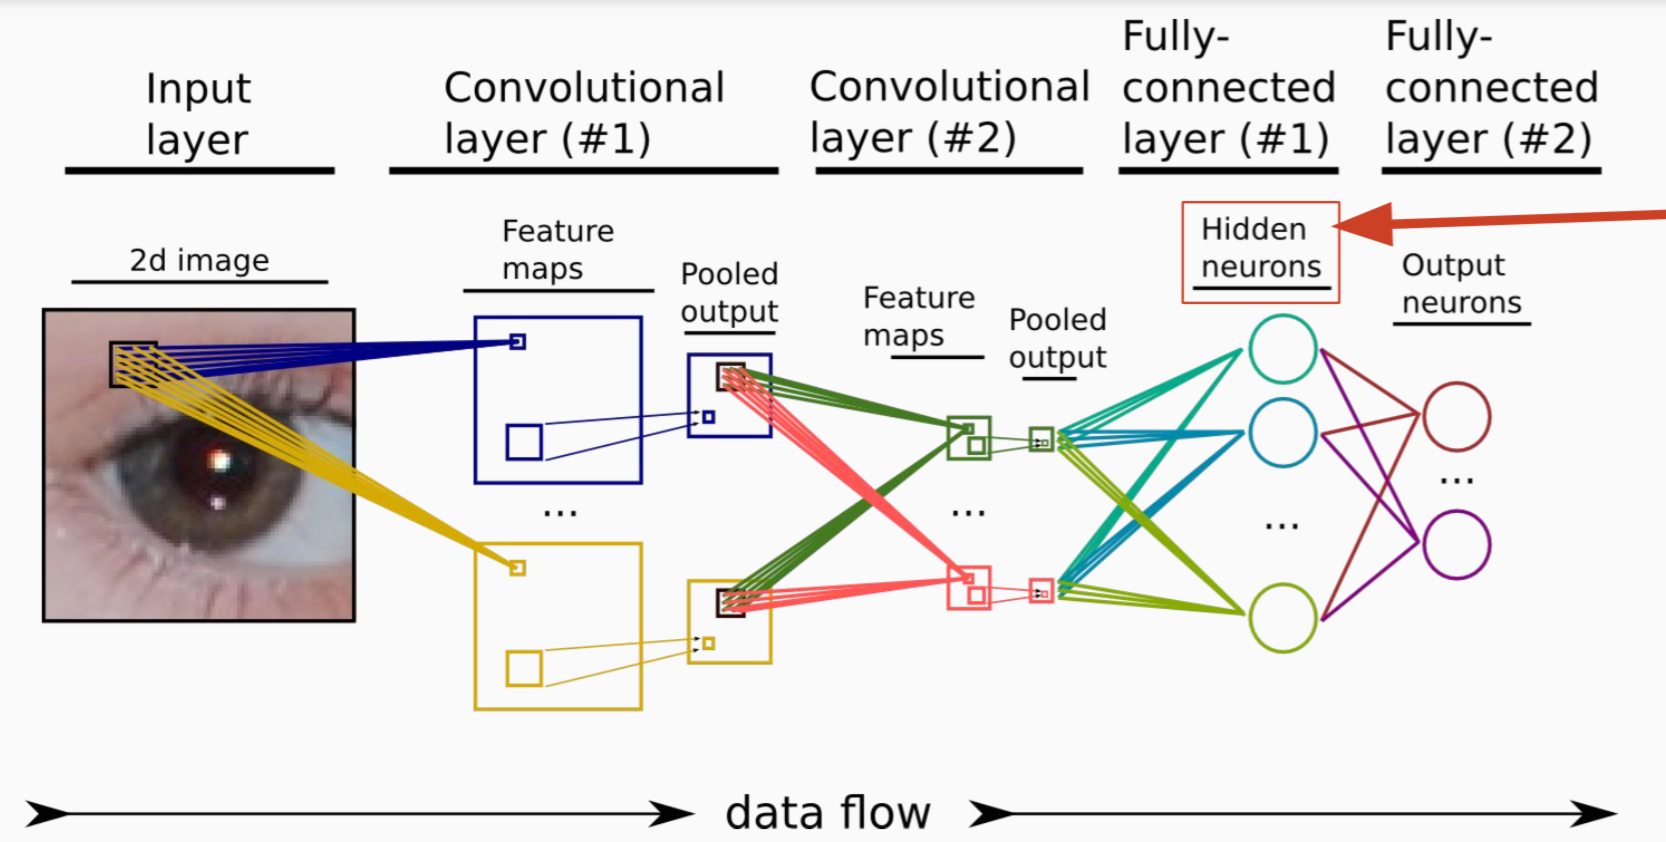
\includegraphics[height=1.05in]{stuff/nn_flow.jpg}}

\only<5>{$\quad\;\;$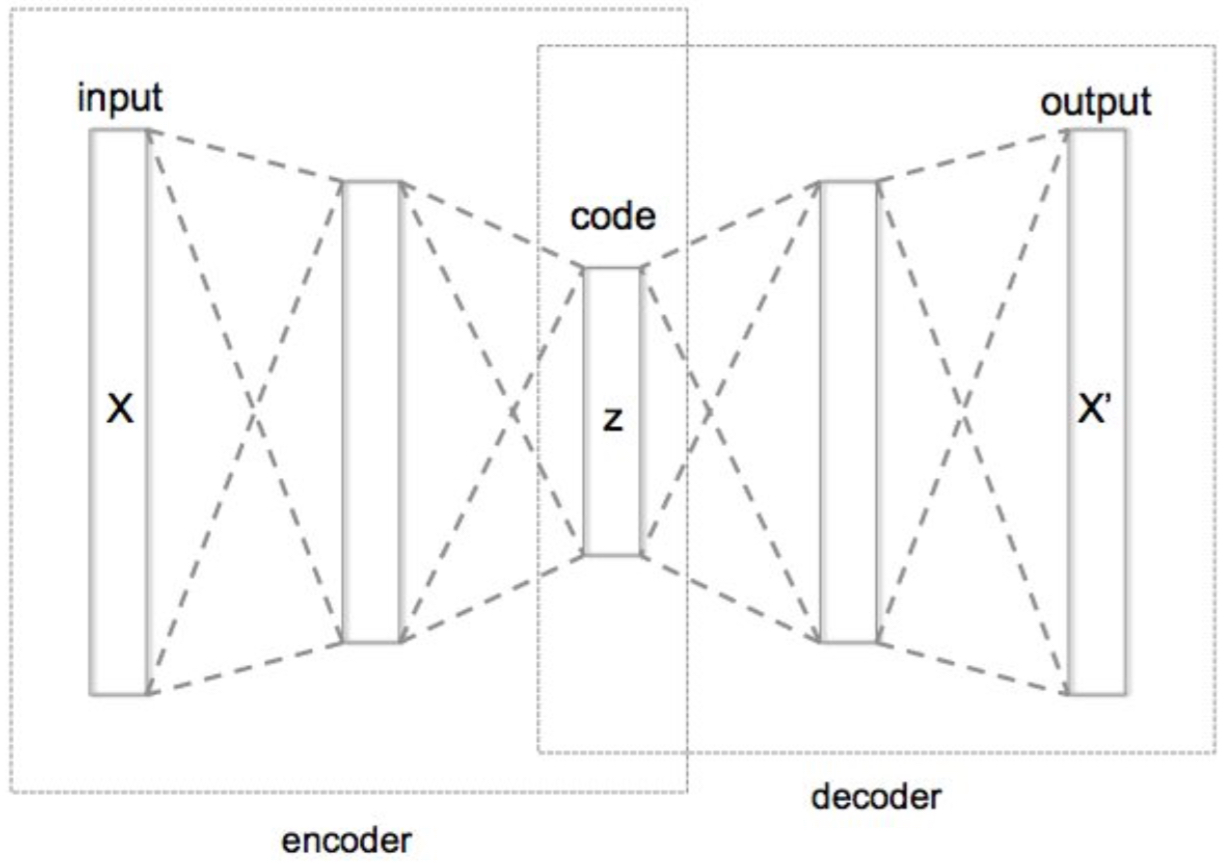
\includegraphics[height=1.3in]{stuff/autoencoder.jpg}}

\only<6->{$\quad$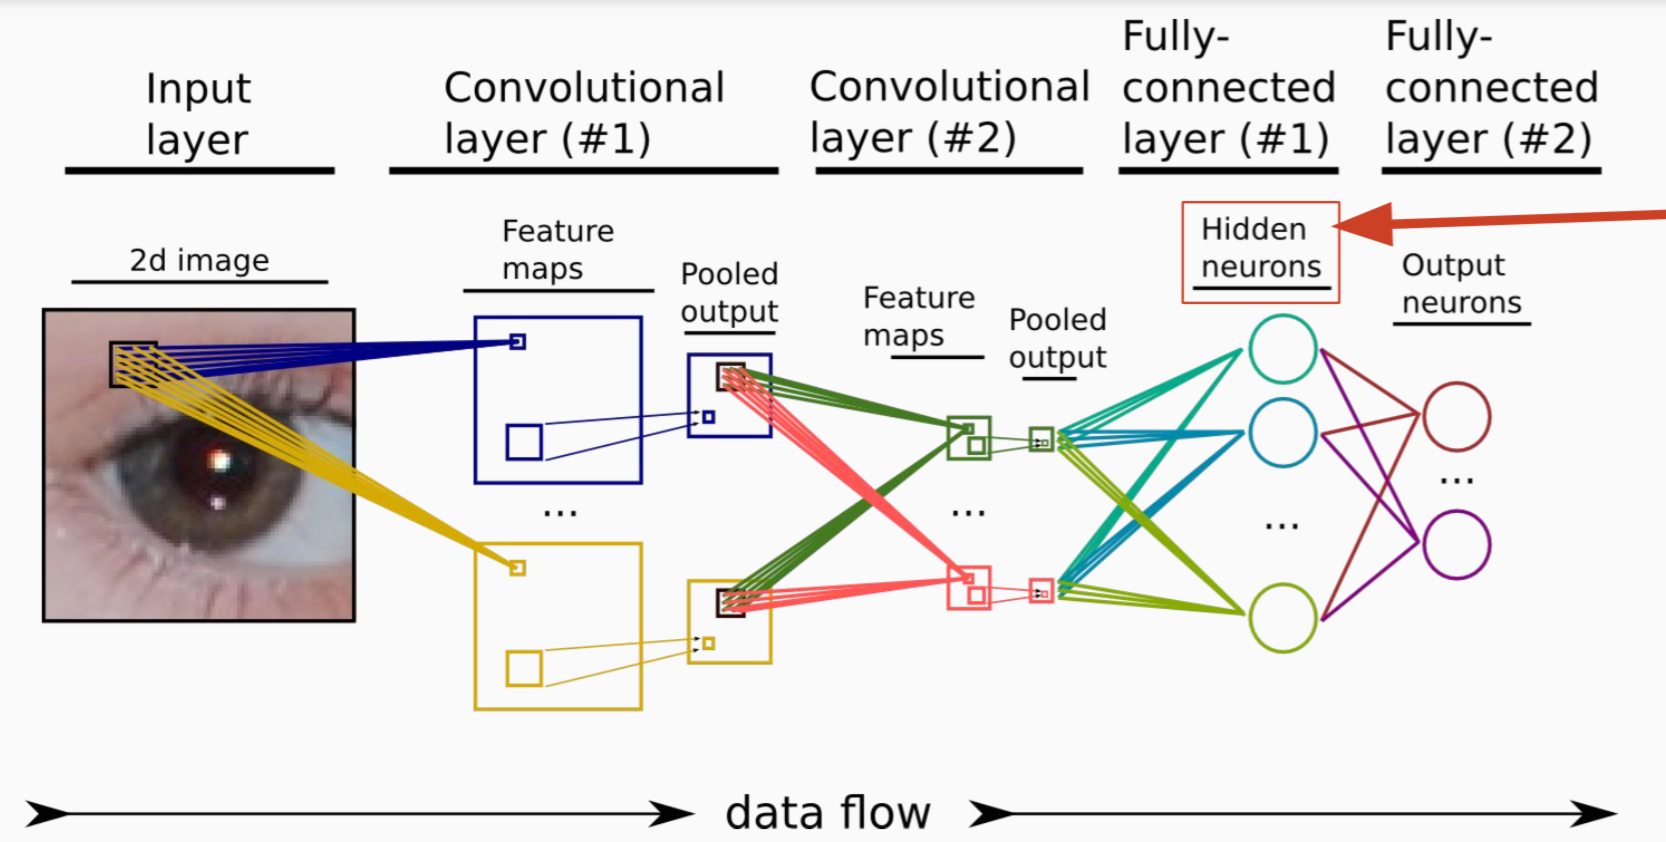
\includegraphics[height=1.05in]{stuff/nn_flow.jpg}}

\end{column}
\end{columns}

}




\frame
{
 \frametitle{Singular Value Decomposition (SVD)}

\footnotesize
$\quad\quad\quad\quad n \times p \quad\quad\quad\quad\quad\quad n \times (q<n) \;\;\; \textcolor{gray}{(q<n) \times (q<p)} \;  (q<p) \times p$
\vspace{-.75em}
\normalsize
\begin{figure}
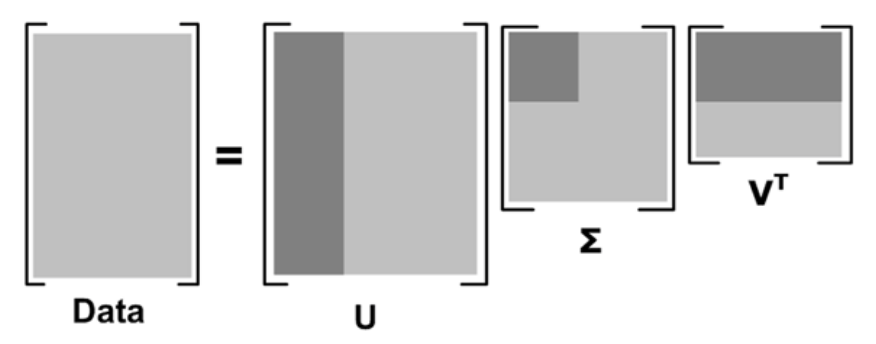
\includegraphics[width=4in]{stuff/svd.png} 
\end{figure}

\begin{itemize}
\item Data: ``standarized'' ${\boldsymbol X}$
\item $U$: Standardized principal component scores
\item $\Sigma$: $\sqrt{eigenvalues}$ on diagonal, 0's off diagonal 
\item $V^T$: Matrix whose rows are the eigenvectors of ${\boldsymbol X}^T{\boldsymbol X}$
\end{itemize}

$$\quad\quad\quad \quad\quad  \underset{1\times 1}{X_{ij'}} \approx \sum_{j=1}^{q<p} \underset{1\times 1}{U_{ij}} \sqrt{\lambda_j} \underset{1\times 1}{V_{jj'}^T} \quad\quad\quad  \textcolor{gray}{\underset{p\times1}{X_{i}} \approx \sum_{j=1}^{q<p} \underset{p\times1}{v_{j}} z_{ij}} $$

}


\frame
{
 \frametitle{Latent Factors}


\vspace{.6em}

\begin{figure}
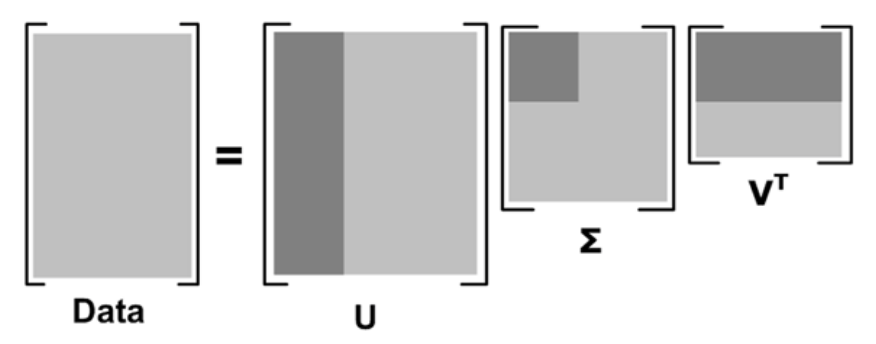
\includegraphics[width=4in]{stuff/svd.png} 
\end{figure}

\vspace{-.4em}


\begin{itemize}
\item Data is the ``phoenotypes'' (features)
\item $U$ is the ``genes'' (factors) driving ``phoenotypes'' (features)
\item $V^T$ is the ``way'' ``genes'' drive  ``phoenotypes''
\item $\Sigma$ controls the strength each ``genes'' influence
\item[]
\item<2-> For some ``high dimensional'' data, e.g., audio, video, these \emph{latent factors}
are the meaningful features associating with $Y$'s
\end{itemize}

}

\frame
{
 \frametitle{Latent Factors}


\begin{figure}
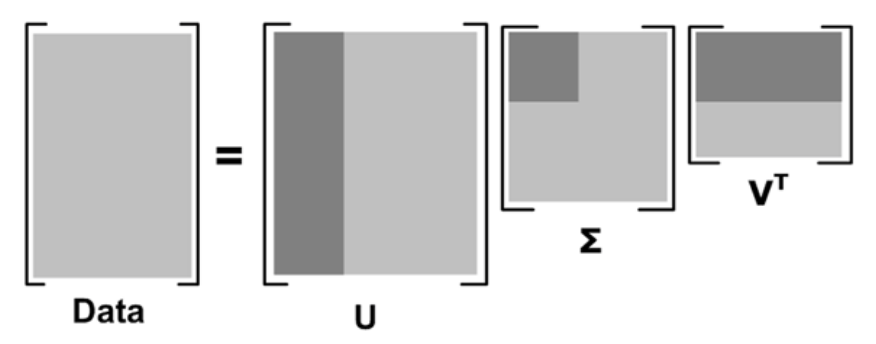
\includegraphics[width=4in]{stuff/svd.png} 
\end{figure}

\vspace{-.425em}

\begin{itemize}
\item When $p > > n$, ${\boldsymbol X}^T{\boldsymbol X}$ is huge
\item SVD doesn't require computation of ${\boldsymbol X}^T{\boldsymbol X}$
\item SVD is a faster, more stable algorithm
\item[]
\item[] $\;$\\$\;$
\end{itemize}
}




\frame
{
 \frametitle{Bonus: Factor Analysis -- genes and phenotypes}

\begin{align*} % requires amsmath; align* for no eq. number
   X_{ij} - \mu_j = {}& \sum_{k=1}^q\beta_{jk} F_{ik} + \epsilon_{ij}
\end{align*}

\begin{tabular}{lllll}
& What & Index & Variable & Note \\
$n$ & samples &  $i = 1, \cdots, n$ &   \\
$p$ & features/sample & $j = 1, \cdots, p$ & $X_{ij}$ & $E[X_{ij}] = \mu_j$\\
$p$ & errors/sample & $j = 1, \cdots, p$ & $\epsilon_{ij}$ &$\overset{iid}{\sim} N(0,\sigma_j)$\\
$q$ & factors/sample & $k = 1, \cdots, q$ & $F_{ik}$ & $\overset{iid}{\sim}$ N(0,1)\\
$p\times q$ & factor loadings &  & $\beta_{jk}$ & Constants\\
\\
\end{tabular}


So for each sample $i$ we have $p$ equations
\begin{align*} % requires amsmath; align* for no eq. number
      X_{i1} - \mu_1 = {}& \beta_{11} F_{i1} + \cdots + \beta_{1k} F_{ik} + \epsilon_{i1} \\
      X_{i2} - \mu_2 = {}& \beta_{21} F_{i1} + \cdots + \beta_{2k} F_{ik}  + \epsilon_{i2}\\
      \vdots \\
      X_{ip} - \mu_p = {}& \beta_{p1} F_{i1} + \cdots + \beta_{pk} F_{ik}  + \epsilon_{ip}\\      
\end{align*}
}

\frame
{
 \frametitle{Bonus: Factor Analysis}

If there are fewer factors $F_{ik}$ than features $X_{ij}$, then we have a reduced
representation of the information in the features. \\${}$\\

For all $j$,  $X_{ij} - \mu_j =  \sum_{k=1}^q\beta_{jk} F_{ik} + \epsilon_{ij}$ 
can be written as
$$\pmb{X}_{i} - \pmb{\mu} = \pmb{\beta} \pmb{F}+ \pmb{\epsilon}$$

Given $X_{ij}$'s, what are $\beta_{jk}, F_{ik},$ and $\epsilon_{ij}$?

\begin{align*} % requires amsmath; align* for no eq. number
      Cov(\pmb{X}) = {}& Cov(\pmb{\beta} \pmb{F} + \pmb{\epsilon}) \\
       = {}&  \pmb{\beta}\pmb{\beta}^T + Cov(\pmb{\epsilon})
\end{align*}	

and the off diagonal entries of $Cov(\pmb{\epsilon})$ should be zero, so we look
for factor loadings $\pmb{\beta}$ to minimize the off diagonal entries of $Cov(\pmb{\epsilon})$.\\${}$\\
      
Given $\pmb{\beta}$, $\pmb{F}$ and $\pmb{\epsilon}$ can be solved for.
The $\pmb{\beta}$ can be adjusted to account for rotations in $\pmb{F}$ that allow for more interpretability. 
      

}

\frame
{
\frametitle{Bonus: Independent Component Analysis (ICA)}

ICA starts out the same way as factor analysis, i.e., 

$$X_{ij} - \mu_j =  \sum_{k=1}^q\beta_{jk} F_{ik}$$ 

but often omits an error term $\epsilon$ as it's an effective procedure w/o it\\${}$\\% $\epsilon$.

Only independence of $F_{ik}$'s is assumed -- not marginal normality;
in fact, the component are chosen sequentially based on  
\emph{extremeness from normality} (as characterized by kurtosis, their $4^{th}$-moment$^*$). \\${}$\\
ICA imagines each $F_{ik}$ gives out independent signals picked up
to varying degrees by different $X_{ij}$ (i.e., \emph{the cocktail party problem}).\\${}$\\

\noindent\rule{1\textwidth}{0.4pt}
\footnotesize{
$^*$$1^{st}$-moment is mean, $2^{nd}$-moment is variance, $3^{rd}$-moment is skew.\\ 
Kurtosis is a measure of ``tail thickness,'' i.e., the extremeness of \\
points that can be generated by the distribution in question.}
}


\frame
{
 \frametitle{Bonus: Graphically}

\begin{columns}
\begin{column}{.5\textwidth}

\vspace{-.75cm}
\begin{figure}
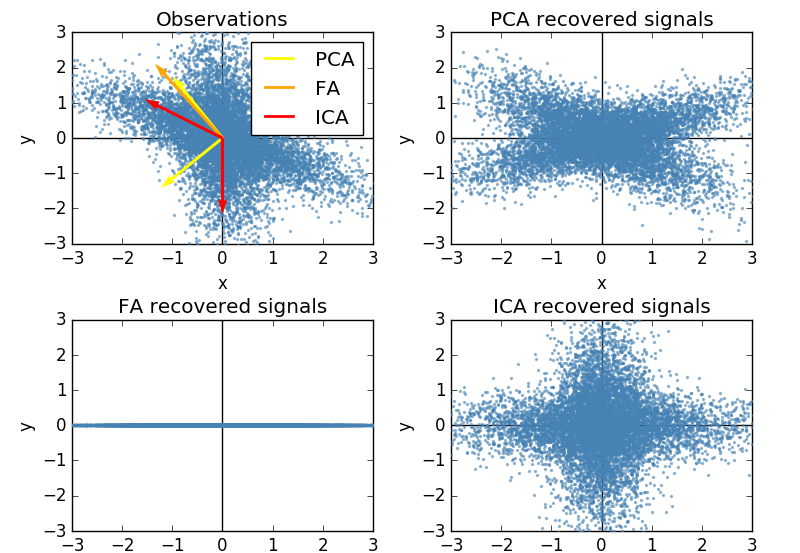
\includegraphics[width=2.25in]{stuff/Q0tvQ.png} 

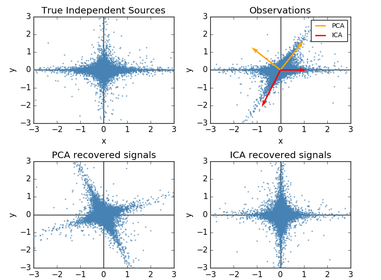
\includegraphics[width=2.3in]{stuff/sphx_glr_plot_ica_vs_pca_thumb.png}
\end{figure}



\end{column}
\begin{column}{.55\textwidth}

Factor analysis finds an underlying uncorrelated lower dimension multivariate normal distribution that, \emph{plus noise}, generates the observed higher dimension data cloud.  E.g., 3D data  generated\\ from a 2D uncorrelated multivariate normal distribution:
\begin{align*} % requires amsmath; align* for no eq. number
      X_{i1} = {}&  1\cdot F_{i1} + 0\cdot F_{i2} + \epsilon_{i1} \\
      X_{i2} = {}& 1\cdot F_{i1} + 0\cdot F_{i2}  + \epsilon_{i2}\\
      X_{i3} = {}& 0\cdot F_{i1} + 1\cdot F_{i2}  + \epsilon_{i3}    
\end{align*}

ICA finds a basis representation \\of the data cloud such that the coordinates of the representation\\ are independent of each other.  

\end{column}
\end{columns}
}


\frame
{
 \frametitle{Bonus: PCA vs. Factor Analysis vs. ICA}
 
 \footnotesize
 
 
The eigenvectors of the feature covariance matrix are an orthogonal basis whose axes capture the directions of maximum variation in the data. The eigenvalues are the relative amounts of variation captured along these axes. Transformation of the data to this coordinate system (i.e., \emph{principal components}) is called PCA.\\${}$\\

PCA is not a generative model like FA -- PCA is purely a representative tool used to describe the data; nonetheless, both methods find orthogonal basis data representations; moreover, the (reduced representation) bases reconstruct the covariance matrix (PCA) or its off-diagonal entries (FA) so for a sufficient number, $q$, of factors and principal components and a relatively uninfluential diagonal,  
 PCA and FA give similar representations.
From here FA latent factors can be ``rotated'' for interpretation. E.g., a latent factor could be lined up with with an ICA component rather than a PCA variance direction.
Unlike ICA, however, the collective set of factor analysis factors remain orthogonal.\\${}$\\

In ICA the underlying basis \emph{is not} orthogonal. This is because rather than targeting an \emph{uncorrelated} representation like FA and PCA, ICA targets an \underline{\emph{independent}} representation. Interestingly, the detection of such a representation requires \emph{exactly} that the underlying representations \emph{not be normal} -- the opposite of the FA assumption.  Independent signals need not be orthogonal features...
\\${}$\\


}




\frame
{
\frametitle{Some Scratch Work}

\footnotesize
\vspace{-.5cm}

\begin{align*} % requires amsmath; align* for no eq. number
   Var(X_{1}) = {}& 3\\
   Var(X_{2}) = {}& 3\\
   Cov(X_{1}, X_{2}) = {}& 2\\
   Var\left(\frac{1}{\sqrt{2}}X_{1}+\frac{1}{\sqrt{2}}X_{2}\right) = {}& \left(\frac{1}{\sqrt{2}}\right)^2Var(X_{1}) + \left(\frac{1}{\sqrt{2}}\right)^2Var(X_{2}) \\
    {}& + 2 \frac{1}{\sqrt{2}}  \frac{1}{\sqrt{2}}Cov(X_{1}, X_{2})\\
   Var\left(\frac{1}{\sqrt{2}}X_{1}+\frac{-1}{\sqrt{2}}X_{2}\right) = {}& \left(\frac{1}{\sqrt{2}}\right)^2Var(X_{1}) + \left(\frac{-1}{\sqrt{2}}\right)^2Var(X_{2}) \\
    {}& + 2 \frac{1}{\sqrt{2}}  \frac{-1}{\sqrt{2}}Cov(X_{1}, X_{2})
\end{align*}

}



\frame
{

$$
\begin{array}{c}
\text{`Directional', Non }\\ 
\text{P.D., \& Singular}\\
\end{array}
\quad
\left[
\begin{array}{ccc}
1 & .6 & .4 \\
.6 & 1 & .4 \\
.4 &  .4 & 1  \\
\end{array}
\right]
\quad
\left[
\begin{array}{ccc}
1 & 1 & 1 \\
1 & 1 & .5 \\
1 &  .5 & 1  \\
\end{array}
\right]
\quad
\left[
\begin{array}{ccc}
1 & 1 & .5 \\
1 & 1 & .5 \\
.5 &  .5 & 1  \\
\end{array}
\right]
$$
}





\frame
{
 \frametitle{PCA as an \emph{approximate} Pythagorean Theorem}

\begin{columns}
\begin{column}{.5\textwidth}
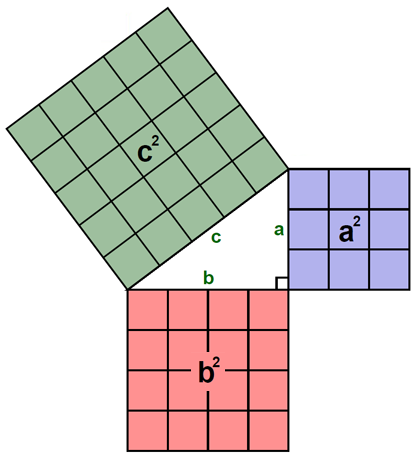
\includegraphics[width=2in]{stuff/pythag2d.png}
\end{column}

\begin{column}{.5\textwidth}
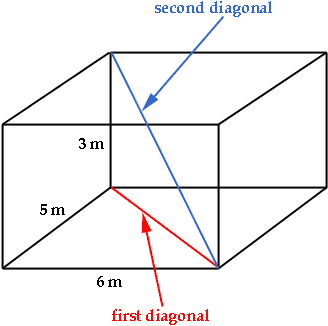
\includegraphics[width=2in]{stuff/pythag3d.jpg}

\begin{align*} % requires amsmath; align* for no eq. number
\textcolor{red}{c^2} = {}& 5^2 + 6^2\\
\textcolor{blue}{c^2} = {}& \textcolor{red}{c^2} + 3^2\\
\textcolor{blue}{c^2} = {}& 5^2 + 6^2 + 3^2
\end{align*}

\end{column}

\end{columns}



 }






\end{document}



\frame
{
 \frametitle{The Sophomore Slump}

{
\fontfamily{<familyname>}\selectfont
\begin{quote}
\tiny
\justify

...or sophomore jinx or sophomore jitters refers to an instance in which a second, or sophomore, effort fails to live up to the standards of the first effort. It is commonly used to refer to the apathy of students (second year of high school, college or university), the performance of athletes (second season of play), singers/bands (second album), television shows (second seasons) and films (sequels/prequels). In the United Kingdom, the ``sophomore slump" is more commonly referred to as ``second year blues", particularly when describing university students. In Australia, it is known as ``second year syndrome", and is particularly common when referring to professional athletes who have a mediocre second season following a stellar debut. The phenomenon of a ``sophomore slump" can be explained psychologically, where earlier success has a reducing effect on the subsequent effort, but it can also be explained statistically, as an effect of the regression towards the mean.

\end{quote}
}

\begin{columns}
\begin{column}{.011\textwidth}
\end{column}
\begin{column}{.6\textwidth}
{
\fontfamily{<familyname>}\selectfont
\begin{quote}
\tiny
\justify

The concept of ``regression'' comes from genetics and was popularized by Sir Francis Galton's late 19th century publication of ``Regression towards mediocrity in hereditary stature.'' Galton observed that extreme characteristics (e.g., height) in parents are not completely passed on to offspring, but rather the characteristics in the offspring ``regress'' towards a mediocre point. By measuring the heights of hundreds of people Galton was able to quantify this ``regression'' and in so doing invented linear regression analysis, thus laying the groundwork for much of modern statistical modeling. The term ``regression'' stuck.
\end{quote}
}
\end{column}
\begin{column}{.4\textwidth}
\vspace{.1in}
\hspace*{-.39in}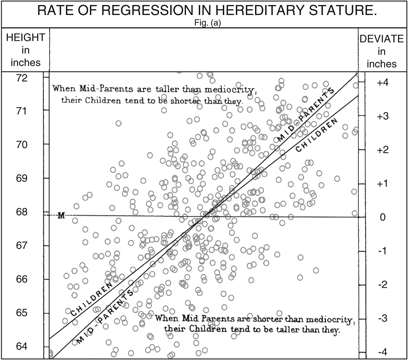
\includegraphics[width=1.55in]{stuff/galton.jpg} 

\end{column}
\end{columns}

% that the offspring of parents who lie at the tails of the distribution will tend to lie closer to the mean of the distribution. 

}

\frame
{
\normalsize
 \frametitle{Objectives}
\begin{itemize}
\item Terminology 
\item Least squares fit
\item Normal distribution theory  
\item Coefficient testing
\item Linear models and Multiple variables and Alternatives
\item Model fit and Model selection
\item Model diagnostics and Model evaluation
\end{itemize}

}

\frame
{
 \frametitle{Linear Models and Regression Terminology}


\vspace{-.25em}
\begin{itemize}
\item[]<2->\textcolor{red}{Outcome / Response / Label / Dependent/Endogenous Var.}
\item $Y_i = \beta_0 + x_i\beta_1 + \epsilon_i, \epsilon_i \overset{\tiny i.i.d.}{\sim}  Normal(0,\sigma^2)$
\item[]<2->  \hspace{4.25em}  \textcolor{red}{Feature / Covariate / Independent/Exogenous Var.}

\vspace{30em}${}$\\

\end{itemize}

}


\frame
{
 \frametitle{Linear Models and Regression Terminology}


\begin{itemize}
\item[]<1-> \hspace{4.5em}   \textcolor{red}{Coefficient} 
\item $Y_i = \beta_0 + x_i\beta_1 + \epsilon_i, \epsilon_i \overset{\tiny i.i.d.}{\sim}  Normal(0,\sigma^2)$
\item[]<1->  \hspace{1.75em}  \textcolor{red}{Intercept   \hspace{2.35em} Error \hspace{2.5em} Noise}\\${}$\\

\vspace{-1em}
\onslide<2->{\includegraphics[width=2.5in]{stuff/Regression1.png}}

\item[]<4-> \textcolor{red}{Fitted/Predicted value \hspace{1em} Residual Standard Error (RSE)}
\item<3-> $ Y_i = \hat\beta_0 + x_i\hat\beta_1 + \hat \epsilon_i, \hat \sigma^2 = \frac{\sum_{i=1}^n \hat \epsilon_i^2}{n-p-1}  \quad (p = \# of \; coefficients)$
\item[]<4->   \hspace{7em} \textcolor{red}{Residual }


\onslide<5->{\hspace{2.5em}\includegraphics[width=2in,height=.75in]{stuff/fit1.png}}

\end{itemize}

}



\frame
{
 \frametitle{Least Squares Fit}

\begin{itemize}

\item $ Y_i = \hat\beta_0 + x_i\hat\beta_1 + \hat \epsilon_i$
\item[] 
\item[]<2->  $[\hat \beta_0,\hat \beta_1] = \underset{[\beta_0, \beta_1]}{argmin} \sum_{i=1}^n \hat \epsilon_i^2 = 
\underset{{\boldsymbol\beta}}{argmin} \sum_{i=1}^n (Y_i - \textbf{x}_i^T{\boldsymbol\beta})^2$\\
\footnotesize
where $\textbf{x}_i^T = [1,x_i]$ and $\textbf{${\boldsymbol\beta}$} = \left[\begin{array}{c} \beta_0\\ \beta_1\end{array}\right]$

\item[]<3-> 
$$\sum_{i=1}^n ( Y_i - \textbf{x}_i^T{\boldsymbol\beta})^2 = (\textbf{Y} - \textbf{x}{\boldsymbol\beta})^T(\textbf{Y} - \textbf{x}{\boldsymbol\beta})$$

\footnotesize
where $\textbf{Y}^T =  [Y_1,Y_2,\cdots,Y_n]$ and $\textbf{x}^T =  \left[\begin{array}{cccc}1&1&\cdots&1\\x_1&x_2&\cdots&x_n \end{array}\right]$

\item[]<4-> \begin{align*}
%\frac{d}{d\hat{\boldsymbol\beta}}
\nabla_{{\boldsymbol\beta}} {} & {\boldsymbol\beta}^T(\textbf{x}^T\textbf{x}) {\boldsymbol\beta}  -2 \textbf{Y}^T \textbf{x}{\boldsymbol\beta}   + \textbf{Y}^T\textbf{Y}\\
=  {} &2 (\textbf{x}^T\textbf{x}) {\boldsymbol\beta}  - 2 \textbf{Y}^T\textbf{x} \quad\quad \textcolor{gray}{\text{(set to \textbf{0} to minimize)}}\\ 
\Longrightarrow {} & \hat{\boldsymbol\beta}  = (\textbf{x}^T\textbf{x})^{-1}  \textbf{x}^T\textbf{Y} \Longrightarrow 
\text{fitted values } \hat {\boldsymbol Y}  =  \textbf{x}\hat {\boldsymbol\beta}
\end{align*}

\end{itemize}
}


\frame
{
 \frametitle{Least Squares Fit \emph{bonus}}

\begin{enumerate}
\item In simple linear regression the $\underset{{\boldsymbol\beta}}{argmin}  (\textbf{Y} - \textbf{x}{\boldsymbol\beta})^T(\textbf{Y} - \textbf{x}{\boldsymbol\beta})$ is
\begin{align*}
\hat \beta_0 = {}& \bar Y -  \hat \beta_1 \bar x \\
\hat \beta_1 = {}& \frac{\sum_{i=1}^n (Y_i - \bar Y) (x_i - \bar x)}{\sum_{i=1}^n (x_i - \bar x)^2} = \frac{R_{xY}S_Y}{S_x}\\
\end{align*}
 
\item<2-> Maximum likelihood estimation (MLE) is equivalent
\begin{align*}
{} & \underset{{\boldsymbol\beta}}{argmax} \prod_{i=1}^n \frac{1}{\sqrt{2\pi \sigma^2}} e^{-\frac{1}{2\sigma^2}(Y_i-\textbf{x}_i^T{\boldsymbol\beta})^2}\\
= {} & 
\underset{{\boldsymbol\beta}}{argmax} (2\pi \sigma^2)^{-\frac{n}{2}} e^{-\frac{1}{2\sigma^2}(\textbf{Y} - \textbf{x}{\boldsymbol\beta})^T(\textbf{Y} - \textbf{x}{\boldsymbol\beta})}\\
= {} & 
\underset{{\boldsymbol\beta}}{argmax} -\frac{n}{2}\log(2\pi \sigma^2) -\frac{1}{2\sigma^2}(\textbf{Y} - \textbf{x}{\boldsymbol\beta})^T(\textbf{Y} - \textbf{x}{\boldsymbol\beta})\\
= {} & 
\underset{{\boldsymbol\beta}}{argmin} (\textbf{Y} - \textbf{x}_i{\boldsymbol\beta})^T(\textbf{Y} - \textbf{x}{\boldsymbol\beta})
\end{align*} 
\end{enumerate}
}


\frame
{
 \frametitle{Outliers}

\begin{figure}
\centering
\includegraphics[width=3.5in]{stuff/outliers2.png}
\end{figure}
}

\frame
{
 \frametitle{Leverage}
The \emph{hat} matrix $H$ ``puts the hat on ${\boldsymbol Y}$'': \textcolor{gray}{$H$ projects ${\boldsymbol Y}$ onto $\hat {\boldsymbol Y}$ -- the (least squares) closest vector (to ${\boldsymbol Y}$) in the column space of $x$ }

\begin{columns}
\begin{column}{.4\textwidth}
\begin{align*}
{}\\
H = {} & \textbf{x}(\textbf{x}^T\textbf{x})^{-1}  \textbf{x}^T\\
\hat {\boldsymbol Y}  = {} & \textbf{x}(\textbf{x}^T\textbf{x})^{-1}  \textbf{x}^T\textbf{Y}\\
 = {} & H\textbf{Y}\\{}\\
\end{align*}
\end{column}
\begin{column}{.6\textwidth}
\onslide<2-> \includegraphics[width=2in]{stuff/outliers5.png}\\${}$
\end{column}
\end{columns}

\vspace{-1.5em}
\begin{itemize}
\item<2-> Diagonal element $H_{ii} \in [0, 1]$, and $\sum_{i=1}^n H_{ii} = rank(\textbf{x})$
\item<2-> $H_{ii}$ shows much $\hat Y_i$ depends on $Y_i$, however
\item<2->[] \textcolor{gray}{$H_{ii}$ actually measures ``extremeness'' of $x_i$} 
\item<2-> Relative comparison of $H_{ii}$'s id.'s ``high leverage observations''  
\item<2->[] \textcolor{gray}{$H_{ii}$ is called the \emph{leverage} of observation $i$}
\end{itemize}


}


\frame
{
 \frametitle{Influential Data Points}

%``Student's t-distributioned'' 
Studentized Residuals have a t-distribution

\begin{columns}
\begin{column}{.4\textwidth}

$$ r_i = \frac{\hat \epsilon_i}{\hat \sigma \sqrt{1-h_{ii}} }$$ \\${}$\\${}$

\end{column}
\begin{column}{.6\textwidth}
\hspace{3.5em}\includegraphics[width=1.5in]{stuff/hl_regress_confiv.png}
\end{column}
\end{columns}

${}$\\${}$\\
%\frac{\text{residual}_i}{\text{RSE}}

\onslide<2->
Influential data points $i$ may have $D_i >$ 
$\{ 3 \times \bar D, 1, 4/n, F_{p,n-p}^{1-\alpha}\}$

\begin{columns}
\begin{column}{.4\textwidth}

\begin{align*}
D_i =& \frac{\sum_{j=1}^n \left(\hat y_j - \hat y_{j(-i)}\right)^2}{\hat \sigma^2p}\\
=& \frac{\hat \epsilon_i}{\hat \sigma^2p}\frac{h_{ii}}{(1-h_{ii})^2}\\{}
\end{align*}

\end{column}
\begin{column}{.6\textwidth}
\onslide<2-> \includegraphics[width=2.5in]{stuff/cooks2.png}
\end{column}
\end{columns}
}

\frame
{
 \frametitle{Regression Diagnostics}

Outliers\textcolor{white}{g}\only<2->{affecting estimates of the residual variance}:
\hspace*{-2.5em}\includegraphics[width=4.75in]{stuff/outliers.png}

High Leverage Points \only<2->{affecting the fitted value predictions}:
\hspace*{3em}\includegraphics[width=3.25in]{stuff/outliers4.png}

}


\frame
{
 \frametitle{\emph{Regression is Multivariate Normal (MVN)}\\
 $\quad\quad\quad$ (inference in regression is based on this normality)}
 
 \setlength{\leftmargini}{-10pt}

\begin{align*}
f(\textbf{Y}|\textbf{x},{\boldsymbol\beta}, \sigma^2) = {} & \prod_{i=1}^n f(Y_i|\textbf{x}_i,{\boldsymbol\beta}, \sigma^2) \\
\onslide<2->{= {} & \prod_{i=1}^n N(\textbf{x}_i^T{\boldsymbol\beta}, \sigma^2)} \\
\onslide<2->{= {} & \prod_{i=1}^n \frac{1}{\sqrt{2\pi \sigma^2}} e^{-\frac{1}{2\sigma^2}(Y_i-\textbf{x}_i^T{\boldsymbol\beta})^2}}\\
\onslide<2->{ = {} & (2\pi \sigma^2)^{-\frac{n}{2}} e^{-\frac{1}{2\sigma^2}(\textbf{Y} - \textbf{x}{\boldsymbol\beta})^T(\textbf{Y} - \textbf{x}{\boldsymbol\beta})} \;\; \textcolor{gray}{= MVN(\textbf{x}{\boldsymbol\beta},\sigma^2I)}} \\ {} \\
 \onslide<3->{\propto {} & e^{-\frac{1}{2\sigma^2}({\boldsymbol\beta} - (\textbf{x}^T\textbf{x})^{-1}  \textbf{x}^T\textbf{Y} )^T \textbf{x}^T\textbf{x} ({\boldsymbol\beta} - (\textbf{x}^T\textbf{x})^{-1}  \textbf{x}^T\textbf{Y})}}\\ 
 \onslide<3->{= {} & (2\pi \sigma^2)^{-\frac{n}{2}} e^{-\frac{1}{2\sigma^2}({\boldsymbol\beta} -  \hat {\boldsymbol\beta})^T \textbf{x}^T\textbf{x} ({\boldsymbol\beta} -  \hat {\boldsymbol\beta})}}\\ 
 \onslide<3->{\Longrightarrow {} & f(\hat {\boldsymbol\beta} |\textbf{x}, {\boldsymbol\beta}, \sigma^2) = MVN\left({\boldsymbol\beta},\sigma^2(\textbf{x}^T\textbf{x})^{-1}\right)} \\
\end{align*} 
}

\frame
{
 \frametitle{A SERIOUSLY MAJOR TRANSITION JUST HAPPENED}

I just added more feature variables without telling you...

}


\frame
{
 \frametitle{Multivariate Regression}
 
% \scriptsize
%That seriously major transition that just happened that you didn't even notice?
 %\normalsize
 
\begin{align*}
Y_i = {}& \beta_0+\beta_1x_{i1} + \cdots + \beta_px_{ip} + \epsilon_i,  \;  \epsilon_i \overset{\tiny i.i.d.}{\sim}  \textrm{N}(0,\sigma^2)\\{}\\
 {\boldsymbol Y} \sim {} &  \textrm{MVN}(\textbf{x}{\boldsymbol\beta},\sigma^2I)\\{}\\
\tiny
\left[\begin{array}{c} Y_1 \\ Y_2 \\ Y_3 \\ \vdots\\ Y_n \end{array} \right] 
= {} & \tiny{\Large \text{$MVN$}} \left(
\left[\begin{array}{ccccc} 1 & x_{11} & x_{21} &\cdots & x_{p1}\\
1 & x_{12} & x_{22} & \cdots & x_{p2}\\ 
1 & x_{13} & x_{23} & \cdots & x_{p3}\\ 
\vdots & \vdots & \vdots & \ddots & \vdots\\ 
1 & x_{1n} & x_{2n} & \cdots & x_{pn}
 \end{array} \right]  
 \left[\begin{array}{c}\beta_0 \\ \beta_1 \\ \beta_2 \\ \vdots\\ \beta_p \end{array} \right]_,
 \left[\begin{array}{cccc}\sigma^2&0 & \cdots & 0\\ 
0 &\sigma^2&  \cdots & 0\\
\vdots &\vdots&  \ddots & \vdots\\
0 & 0 &   \cdots & \sigma^2\\ \end{array}\right]\right)\end{align*}

\begin{itemize}
\item[]
\item<2-> It's just a (multivariate) normal distribution 
\item<3-> with a \emph{linear model} component for the mean \onslide<4->{just} \onslide<5->{like} \onslide<6->{before}
\item[]
\item<4-> Interpret: %$\text{E}[Y] = \beta_0 + \beta_1X_1 + \beta_2X_2 + \beta_{2^2}X_2^2 + \beta_{13}X_1X_3 $
is it possible to ``vary one $X$ and hold all others constant''?
\end{itemize}

}



\frame
{
 \frametitle{Assumptions, violations, and remedial measures}


$$Y_i = \beta_0+\beta_1x_{i1} + \cdots + \beta_px_{ip} + \epsilon_i,  \;  \epsilon_i \overset{\tiny i.i.d.}{\sim} \textrm{N}(0,\sigma^2)$$
 
\begin{columns}
\begin{column}{.33\textwidth}
\vspace{-1.5in}
\begin{itemize}
\item<2-> Normality
\item<4-> Homoskedasticity
\item<6-> Independence
\item<7-> Linear form
\item<8-> Fixed $x$'s
\end{itemize}
\end{column}
\begin{column}{.67\textwidth}
%\vspace{.25in}
\begin{itemize}
\item<2-3> [] 
\includegraphics[width=2in]{stuff/qq1.png}\\ % statistical results compromised -- can perhaps transform
Q-Q Plot\\${}$\\
\textcolor{gray}{Hypothesis testing depends on distributional assumptions}
 % transform 
\vspace{-2.64in}
\item<3>[] 

\textcolor{white}{llllllll}\includegraphics[width=1.715in,height=1.51in]{stuff/qq2.png}

\vspace{-1.7in}
\item<4-5> [] 
\includegraphics[width=2in]{stuff/hets1.png}\\ % statistical results compromised -- can perhaps transform
Residuals versus Fitted Values\\${}$\\
\textcolor{gray}{Box-Cox transformations $\frac{Y^\lambda-1}{\lambda}$ can help}
 % transform 
\vspace{-2.75in}
\item<5>[] 
\includegraphics[width=2in]{stuff/hets2.png}
\item<6>[] 
\vspace{-1.5in}
$\text{Cov}[{\boldsymbol Y} - {\boldsymbol X\beta}]$
%= \frac{({\boldsymbol Y} - {\boldsymbol X\beta})({\boldsymbol Y} - {\boldsymbol X\beta})^T}{n-p-1}$\\${}$\\
%$\quad\quad\quad\quad\quad\quad
$\approx\left[\begin{array}{cccc}\sigma^2&0 & \cdots & 0\\ 
0 &\sigma^2&  \cdots & 0\\
\vdots &\vdots&  \ddots & \vdots\\
0 & 0 &  \cdots & \sigma^2\\ \end{array}\right]$

\item<7>[] 
\vspace{-1.25in}
\includegraphics[width=2in]{stuff/resids.png}\\ % statistical results compromised -- can perhaps transform
Residuals versus Feature Values\\${}$\\
\textcolor{gray}{``All models are wrong, some are useful'' -- George Box}


\end{itemize}
\end{column}
\end{columns}
%fits.png


% stats people care about diagnostics -- do you?
%\item Challenges interpreting coefficients? 

}



\frame
{
 \frametitle{Multicollinearity and the Variance Inflation Factor (VIF)}

\onslide<1->{\textcolor{gray}{And when you have any number of covariates (features)...}}

\begin{itemize}
\item[] 
$$\hat {\boldsymbol\beta} \sim MVN\left({\boldsymbol\beta},\sigma^2(\textbf{x}^T\textbf{x})^{-1}\right)$$
\item<2>[] 
\begin{figure}
\centering
\includegraphics[width=2.4in]{stuff/VIF2.png}
\end{figure}
\vspace{-2.5in}
\item<3>[] 
\begin{figure}
\centering
\includegraphics[width=3.5in]{stuff/VIF1.png}
\end{figure}
\vspace{-2.25in}
\item<4->[]${}$\\${}$\\

 $$\widehat{\text{Var}}[\hat \beta_j] = \frac{\hat \sigma^2}{(n-1)  \widehat{\text{Var}}[X_j]}\cdot \textcolor{red}{\frac{1}{1-R^2_j}} \quad\quad \textcolor{red}{\text{[VIF]}}$$ 

where $R^2_j$ is the $R^2$ of $X_j$ regressed on all the other $X$'s\\${}$\\

\item<5->[] \textcolor{gray}{Could make an array of VIFs...?}
\item<6->[] \textcolor{gray}{Centering $X$'s can decorrelate $X$ and $X^2$...}
\item<7->[] \textcolor{gray}{Scaling $X$'s (putting $X$'s on the same scale) helps numerically}

\end{itemize}

%\item The role of rank($X$) and multicollinearity? % centering/scaling

}


\frame
{
 \frametitle{Model Fit}


\begin{table}[h!]
\centering
\begin{tabular}{|c|c|}
\hline
&\\
 Residual Variation  & Total Variation  \\
&\\
$RSS = \sum(Y_i - \hat Y_i)^2 \textcolor{gray}{= \sum \hat \epsilon_i^2}$ & $TSS = \sum(Y_i - \bar Y)^2 $ \\
 & $\textcolor{white}{RSEEEEEee}  \textcolor{gray}{= RSS + \sum( \hat Y_i - \bar Y )^2}$ \\
&\\ \hline
&\\
Residual Standard Error & Proportion of Variance Explained\\
&\\
$RSE = \sqrt{\frac{1}{n-p-1}RSS}$ & $R^2 = \frac{TSS - RSS}{TSS}$ \\
$\textcolor{white}{RSEEEE} = \sqrt{\frac{\sum(Y_i - \hat Y_i)^2}{n-p-1}}$ &$\textcolor{white}{R} = 1-\frac{RSS}{TSS}$\\
&\\ \hline
\multicolumn{2}{|c|}{$F$-test}\\
\multicolumn{2}{|c|}{$F =  \frac{(TSS - RSS)/p}{RSS/(n-p-1)} = \frac{\sum(\hat Y_i -\bar Y )^2/p}{\sum( Y_i -\hat Y )/(n-p-1)}$}\\ 
\multicolumn{2}{|c|}{${}$}\\\hline
\end{tabular}
\end{table}

}

\frame
{
 \frametitle{Decomposition of Total Variation}

\begin{figure}
\centering
\includegraphics[width=4in]{stuff/sspartition.png} 
\end{figure}
\vspace{-2em}

\begin{align*}
TSS = {} & \sum(Y_i - \bar Y)^2 =  \sum( Y_i - \hat Y_i + \hat Y_i - \bar Y )^2 \\
= {} & \sum( Y_i - \hat Y_i )^2 + 2 \sum ( Y_i - \hat Y_i )( \hat Y_i - \bar Y ) +\sum( \hat Y_i - \bar Y )^2 \\
= {} & \sum( Y_i - \hat Y_i )^2 + 2 \sum \hat \epsilon_i ( \hat Y_i - \bar Y ) + \sum( \hat Y_i - \bar Y )^2 \\
{} &\textcolor{gray}{\quad\quad\quad\quad\quad\sum \hat \epsilon_i = 0 \uparrow \;\;\; \uparrow \sum \hat \epsilon_i\hat Y_i = 0}\\
= {} & \sum( Y_i - \hat Y_i )^2 + \sum( \hat Y_i - \bar Y )^2 =  RSS + \sum( \hat Y_i - \bar Y )^2 
\end{align*}

}


\frame
{
 \frametitle{Model Selection}

\begin{itemize}
\item<1-> $R^2$ (model fit) is insufficient -- more features means larger $R^2$
\item<2-> Spuriously improving model fit to data is called \emph{overfitting}
\item<3-> \underline{We want model fits to generalize to \emph{population} phenomenon} 
\item[]
\item<4-> Classical Model Selection Criterion\\${}$\\
\begin{tabular}{|rl|l|}
\hline & &\\
Mallow's $C_p$ & $\frac{1}{n}(RSS + 2p\hat\sigma^2)$ & \\
&&\\
$AIC$ & $-2\log L+2p$          & $D_M = - 2\text{log}f(Y|\hat \theta^{M_p})$ \\
&                                            &  $ \textcolor{white}{D_M = } + 2\text{log}f(Y|Y)$ \\             
$BIC$ & $-2\log L+p\log n $  & \\
&&\textcolor{gray}{$D_M \overset{\tiny approx.}{\sim}   \chi^2_{n-p-1}$} \\
$Adjusted \; R^2$ & $1 - \frac{RSS/(n-p-1)}{TSS/(n-1)}$& \\
&&\\\hline 
\end{tabular}
\end{itemize}

}





\frame
{
 \frametitle{Testing: an example with simple linear regression}
 
 \setlength{\leftmargini}{-10pt}
\vspace{-1.5em}
\begin{itemize}
\item[] 
\begin{align*} 
f(\textbf{Y}|{\textbf{x}, \boldsymbol\beta}, \sigma^2) = {} & MVN(\textbf{x}{\boldsymbol\beta},\sigma^2I) \\
 \Longrightarrow f(\hat {\boldsymbol\beta} | \textbf{x}, {\boldsymbol\beta}, \sigma^2) = {} & MVN\left({\boldsymbol\beta},\sigma^2(\textbf{x}^T\textbf{x})^{-1}\right) 
\end{align*} 


\item[]<2-> For simple linear regression then 

$$\hat {\boldsymbol\beta} \sim MVN\left( \left[\begin{array}{c} \beta_0 \\ \beta_1 \end{array}\right]_{\Large,} 
\frac{\sigma^2}{n \sum (x_i - \bar x)^2} \left[\begin{array}{cc} \sum x_i^2 & - \sum x_i\\ - \sum x_i&  n \end{array} \right] \right) $$

\item[]<3->
where 

$$\textcolor{gray}{\hat \beta_0 = \bar Y -  \hat \beta_1 \bar x \quad
\hat \beta_1 = \frac{\sum_{i=1}^n (Y_i - \bar Y) (x_i - \bar x)}{\sum_{i=1}^n (x_i - \bar x)^2} = \frac{R_{xY}S_Y}{S_x}}$$

$$\text{Var}(\hat \beta_1) = \sigma^2\frac{1}{\sum_{i=1}^n (x_i - \bar x)^2} \quad
\text{Var}(\hat \beta_0) = \sigma^2\left[\frac{1}{n} + \frac{\bar x^2}{\sum_{i=1}^n (x_i - \bar x)^2} \right]$$
%\vspace{.1em}

\item[]<4-> 
$$\textcolor{gray}{\text{SE}(\hat \beta_0) = \sqrt{\text{Var}(\hat \beta_0)} \quad \text{SE}(\hat \beta_1) = \sqrt{\text{Var}(\hat \beta_1)}}$$
\end{itemize}
}




\frame
{
 \frametitle{Testing \emph{Extra Credit}}

\begin{itemize}
\item
What is $\text{Var}(\hat Y_0)$? \textcolor{gray}{(Suppose we know $\sigma^2$)}
%\item[] % use general variance formula
%\item[] % get (\sigma^2/n)*(sum(x_i-x_0)^2/sum(x_i-\bar x)^2) 
%\item[] % and can also show (with the other formula) that 
%\item[] % get \sigma^2(1/n + (x_0 - \bar)x^2/sum(x_i-\bar x)^2]
\item[] 
\item[] \emph{Hint: $\hat Y_0 = \hat \beta_0 +  x_0\hat \beta_1  $}
\item[] \emph{Hint: $\text{Var}[aX+bY]=\;?$}
\item[]
\item[]
\item[] 
\item
$\text{Var}(Y_0)$? For a \emph{new observation} $Y_0$ according to our model? 
\item[] \textcolor{gray}{(Suppose we know $\sigma^2$)}
\item[] 
\item \emph{Hint: $Y_0 = \hat \beta_0 +  \hat \beta_1 x_0 + \epsilon$}
\end{itemize}
}




 
\frame
{
 \frametitle{Coefficient Testing \emph{in General}}
 
For $\hat{\boldsymbol\beta}  = (\textbf{x}^T\textbf{x})^{-1}  \textbf{x}^T\textbf{Y}$, since (under $H_0$)
$$f(\hat {\boldsymbol\beta} | {\boldsymbol\beta}, \sigma^2) = MVN\left({\boldsymbol\beta}, \sigma^2(\textbf{x}^T \textbf{x})^{-1}\right)$$
we have that 
\onslide<2->{$$\frac{\hat \beta_i - \beta_i}{\text{SE}(\hat \beta_i)} \sim  N(0,1)$$}
\onslide<3->{and if we estimate 
$$\hat \sigma^2 = \frac{(\textbf{Y} - \textbf{x}\hat{\boldsymbol \beta})^T(\textbf{Y} - \textbf{x}\hat{ \boldsymbol  \beta})}{n-p-1}$$
(where $p$ is the number of coefficients) then we have that} 
\onslide<4->{$$\frac{\hat \beta_i - \beta_i}{\text{SE}(\hat \beta_i)} \sim  t_{n-p-1}$$}

\onslide<5->{\textcolor{gray}{And this works for any number of feature variables...}}
%\left({\boldsymbol\beta}

}


\frame
{
 \frametitle{Coefficient Testing \emph{in even more Generality}}

${}$\\${}$\\${}$\\${}$\\
\begin{columns}
\begin{column}{.6\textwidth}
\fbox{\includegraphics[width=2.3in]{stuff/waldVS.png}}
\end{column}
\begin{column}{.55\textwidth}
\vspace{-.075in}

\underline{Wald test}\\
$\frac{(\hat \theta - \theta_0)^2}{Var(\hat \theta)} \overset{\tiny approx.}{\sim} N(0,1) \textcolor{gray}{\text{ under } H_0}$\\${}$

\underline{Likelihood-Ratio (LR) test}\\
$-2ln\left(\frac{L(\theta_0|x)}{{L(\theta|x)}}\right) \overset{\tiny approx.}{\sim} \chi^2_k \textcolor{gray}{\text{ under } H_0}$\\${}$

\underline{Score test} \\
$\frac{\left(\frac{\partial}{\partial \theta } \log L(\theta_0|x)\right)^2}
{-\text{E}\left[\frac{\partial^2}{\partial \theta^2 } \log L(\theta_0|x)\right]} \overset{\tiny approx.}{\sim} \chi^2_1 \textcolor{gray}{\text{ under } H_0}$

\end{column}


\end{columns}
${}$\\${}$\\${}$\\${}$\\
\onslide<2->{\textcolor{gray}{And this works for any number of covariates...}}

}






\frame
{
 \frametitle{Hypothesis Testing for Feature Selection}

\vspace{-1em}
\begin{align*}
\textcolor{gray}{F =} {}& \textcolor{gray}{\frac{(TSS - RSS)/p}{RSS/(n-p-1)} = \frac{\sum(\hat Y_i -\bar Y )^2/p}{\sum( Y_i -\hat Y )/(n-p-1)}} \\{}\\
F \sim  {}& F_{p,n-p-1} \quad \textcolor{gray}{\text{(tests if any coefficient is \emph{non-zero})}} \\ 
\frac{\hat \beta_i - \beta_i}{\text{SE}(\hat \beta_i)} \sim  {} & t_{n-p-1} \quad\quad \textcolor{gray}{\text{(tests if a \emph{specific} coefficient is non-zero*)}}\\
{} &\;\quad\quad\quad\quad \scriptsize \textcolor{gray}{\text{*in the presence of all the others (this is a ``last-in'' test)}}\\
\end{align*}

\vspace{-.6in}
\begin{itemize}
\item<2->[]
\hspace*{.75in}\includegraphics[width=3.5in]{stuff/regtable.png} 
\vspace{-1.6in}
\item<3-> Forward \\Selection\\${}$\\
\item<4-> Backward \\Selection\\${}$\\
\item<5-> Both \\${}$\\
\end{itemize}


}







\frame
{
 \frametitle{Linear Models}

\begin{itemize}
\item Linear model... that sounds too simple...
\item<2->[] 
\hspace*{-.25in}\includegraphics[width=1.75in]{stuff/OLS2.png}
\vspace{-1.75in}
\item<3->[] 
\hspace{1.4in}\includegraphics[width=2.5in]{stuff/spline.png} 
\item[] 
\item<4-> ``Linear'' models are only linear in the coefficients
$$Y_i = \beta_0+\beta_1x_{i1} + \cdots + \beta_px_{ip} + \epsilon_i$$
\item<4-> The $x$'s can be pretty wild... 
\end{itemize}

}

\frame
{
 \frametitle{Linear models that produce ``non-linear'' response surfaces}
 
\begin{itemize}
\item<2-> Higher order terms: $X_1^{\frac{1}{2}},X_1^2, X_1^3$
\item<3-> Qualitative variables: $X_1 \in \{0,1\}, X_1 \in \{a,b,c,d\}$
\item[]<4-> $$ \left[ \begin{array}{c}a\\b\\c\\d\end{array} \right] = \left[ \begin{array}{ccc}0&0&0\\1&0&0\\0&1&0\\0&0&1\end{array} \right] \quad\quad \left[ \begin{array}{c}a\\b\\c\\d\end{array} \right] \textcolor{red}{\not = \left[ \begin{array}{cccc}1&0&0&0\\0&1&0&0\\
0&0&1&0\\0&0&0&1\end{array} \right]} $$


\item<5-> Interactions: $X_1\cdot X_2$ \textcolor{gray}{\emph{(interpretation?)}}
\item[]
\item[]<6-> Step functions
\item[]<6> ${}$\\$Y_i = \beta_j : if \; a_j \leq X_i < b_j$
\item[]<6> 
\vspace{-.75in}
\hspace*{2in}\includegraphics[width=1.75in]{stuff/step.png} 

\vspace{-.825in}
\item[]<7-> Regression Splines\\${}$\\
\item[]<7> 
$\quad\quad\quad Y_i = \left\{\begin{array}{ll} 
\beta_0 + \beta_1X_i + \beta_2X_i^2  + \beta_3X_i^3  +  \epsilon_i & : if  \; X_i \leq c\\
\beta_0^* + \beta_1X_i + \beta_2^*X_i^2  + \beta_3^*X_i^3  +  \epsilon_i & : if \; X_i > c
\end{array} \right. $
\item[]<7-8> 
\vspace{-1in}
\hspace*{1.25in}\includegraphics[width=.7in]{stuff/splines1.png}\includegraphics[width=.7in]{stuff/splines2.png}\includegraphics[width=.7in]{stuff/splines3.png}\includegraphics[width=.7in]{stuff/splines4.png} 
\item[]<8> 
\hspace*{-.525in}$h(X_i,\xi) = \left\{\begin{array}{ll} 
(x - \xi)^3 &:  if \; X_i > \xi \\
0 & :  if  \; X_i \leq \xi 
\end{array} \right.  Y_i = \begin{array}{ll} 
\beta_0 + \beta_1X_i + \beta_2X_i^2  + \beta_3X_i^3   \\
+ \beta_{s1} h(X_i,\xi_1)  + \cdots + \epsilon_i
\end{array} $
\vspace{-.63in}
\item[]<9-> Smoothing Splines  

\vspace{-4.5em}
$\quad\quad\quad\quad\quad\quad\quad\quad\quad\quad$\includegraphics[width=2in]{stuff/spline.png} 

\vspace{-.54em}
$\textcolor{white}{Smooth Spline Splines}\displaystyle\underset{g}{\min} \sum_{i=1}^n (Y_i -g(x_i))^2 + \lambda \int g''(t)^2 dt$
\vspace{1in}



\end{itemize}
 
 %interpretation 
 
% \item Higher order terms -- what does ``linear'' mean? 
% indicator variabales
% interactions

% fancy polynomial splines
% smoothing splines
 
}

\frame
{
\frametitle{Linear models aren't really so ``linear''}

\begin{figure}
\centering
\includegraphics[width=4in]{stuff/spline.png} 
\end{figure}
}

\frame
{
 \frametitle{Other ways to get ``non linear'' response surfaces}
 
 \begin{itemize}
 \item Local Regression (LOESS)
\textcolor{white}{H}\includegraphics[width=3in]{stuff/loess.png} 

 \item<2-> Generalized Additive Models\\${}$\\
\vspace{-.1in}
 \includegraphics[width=3.15in]{stuff/gam.png} 
 \end{itemize}
 
}


\end{document}


\frame
{
 \frametitle{Variance Partitioning and the Variance/Bias Tradeoff}
 
 \footnotesize
For fixed $\hat f(x)$ estimating true $f(x)$
\begin{align*}
\underset{Y}{\text{E}}[(Y-\hat f(x))^2] = {} & \underset{\epsilon}{\text{E}} [(f(x) + \epsilon - \hat f(x))^2] \\
= {} & \underset{\epsilon}{\text{E}} [(f(x) - \hat f(x) + \epsilon)^2 ] \\ 
= {} & \underset{\epsilon}{\text{E}} [(f(x) - \hat f(x))^2] + \underset{\epsilon}{\text{E}} [2(f(x) - \hat f(x))\epsilon]  + \underset{\epsilon}{\text{E}}[\epsilon^2]  \\ 
= {} & (f(x) - \hat f(x))^2 + 2(f(x) - \hat f(x))\underset{\epsilon}{\text{E}} [\epsilon]  + \underset{\epsilon}{\text{E}}[\epsilon^2]  \\ 
= {} & (f(x) - \hat f(x))^2 + \underset{\epsilon}{\text{E}}[\epsilon^2]  \\ 
{} & \quad reducible \quad\; irreducible \\
 reducible \quad\quad\quad\;\;&\\
 \underset{\hat f(x)}{\text{E}}\left[(f(x) - \hat f(x))^2\right] = {} & \underset{\hat f(x)}{\text{E}}\left[\left(f(x) - \underset{\hat f(x)}{\text{E}}[\hat f(x)] + \underset{\hat f(x)}{\text{E}}[\hat f(x)] - \hat f(x)\right)^2\right] \\
= {} & \underset{\hat f(x)}{\text{E}} \left[\left(f(x) - \underset{\hat f(x)}{\text{E}}[\hat f(x)] \right)^2\right] 
 +  \underset{\hat f(x)}{\text{E}}\left[\left(\underset{\hat f(x)}{\text{E}}[\hat f(x)] - \hat f(x)\right)^2\right] \\
& \quad\quad\quad\quad\quad\quad bias \quad\quad\quad\quad\quad\quad\quad\quad\quad variance  \\
\end{align*}
}






